% Output
% dvips userguide_3.3
% ps2pdf userguide_3.3.ps;mv userguide_3.3.pdf userguide_npde3.3.pdf

\documentclass[12pt,a4paper]{article}
\usepackage{epsfig}
%\usepackage{graphicx}
\DeclareGraphicsExtensions{.jpg, .eps}
\DeclareGraphicsRule{.jpg}{eps}{.jpg.bb}{`jpeg2ps -h -r 600#1}
\usepackage{amsmath,amssymb,amsthm,indentfirst,array,bbm}
\usepackage{lscape}
\usepackage{longtable}
\usepackage{dcolumn}
\setlength{\LTcapwidth}{\textwidth} % caption length for longtable

\usepackage[T1]{fontenc}
\usepackage{pslatex}
%\usepackage{calc}

\usepackage{fancyheadings}
%\usepackage{fancyhdr}
%\usepackage{color}
%\usepackage{/home/eco/xtex/Lib/figreport}
%\usepackage{/home/eco/cours/coursR/zemanuel/manuelfig}
\usepackage[dvipsnames]{color}
\usepackage[dvips,colorlinks,hyperindex]{hyperref}

\definecolor{mycol}{rgb}{0.5,0.1,0.6}

\hypersetup{pdftitle="Userguide for npde 3",pdfauthor="Emmanuelle Comets",
linkcolor=mycol,urlcolor=mycol,citecolor=mycol}
%--
%-- Dimensions
%--
\setlength{\topmargin}{-0.5cm}
\setlength{\textheight}{23cm}
\setlength{\textwidth}{17cm} 
\setlength{\oddsidemargin}{-0.5cm}

%Typographie
\renewcommand{\baselinestretch}{1.3}
\renewcommand{\topfraction}{0.99}
\renewcommand{\bottomfraction}{0.99}

\setlength{\itemsep}{0pt}
\parindent 18pt

\def\Y{{\rm Y}}
%\def\var{{\rm var}}
\def\var{\hbox{var}}
\def\npde{{\rm npde}}
\def\tnpde{{\rm tnpde}}
\def\tnpd{{\rm tnpd}}
\def\pde{{\rm pde}}
\def\npd{{\rm npd}}
\def\pd{{\rm pd}}
\def\vec{{\rm vec}}
\def\ypred{{\rm ypred}}
\def\R{{\sf R}}
\def\true{{\sf TRUE}}
\def\false{{\sf FALSE}}


%\makeindex
\begin{document}
\definecolor{violet}{rgb}{0.25,0.1,0.75}
%\definecolor{mycol}{rgb}{0.5,0.1,0.6}

\pagestyle{fancy}
\renewcommand{\headrulewidth}{0pt}
\renewcommand{\footrulewidth}{1pt}
%\renewcommand{\footrulewidth}{0pt}
\lhead{}
\chead{}
\rhead{}
\lfoot{\itshape E. Comets, \today}
\cfoot{User Guide for npde 3.3}
\rfoot{\thepage}

\newcommand{\D}{\displaystyle} \normalsize
\renewcommand{\thetable}{\Roman{Contents}}
\renewcommand{\refname}{References}
\renewcommand{\listfigurename}{{\bfseries \sc Legends for figures}}
\renewcommand{\labelitemi}{$\bullet$}

\parindent 18pt
$\phantom{minime}$

\vskip 3cm
\begin{center}
{\setlength{\baselineskip}{2\baselineskip}
{\Large \bfseries User guide for npde 3.3/3.4}

{\Large \bfseries October 2022}

\bigskip 

{\Large \itshape \bfseries Emmanuelle Comets}

{\large \itshape \bfseries Contributors to the npde package: Karl Brendel, Marc Cerou, Thi Huyen Tram Nguyen,  Romain Leroux, France Mentr\'e}

\bigskip
{\it
INSERM, IAME UMR 1137, Paris, France

Universit\'e de Paris, Paris, France.
}
\par}
\end{center}

\vskip 8cm % TODO: bookdown !
% \begin{center}
% {\large \bfseries npde website: www.npde.biostat.fr}
% \end{center}

\newpage
%{\setlength{\baselineskip}{0.8\baselineskip}
\tableofcontents
%}\par
\newpage

\hskip 18pt  This is the User's guide for the add-on package {\sf npde} (version 3.3, October 2022) for the {\sf R} 
language. It is distributed in the \texttt{inst} directory of the package. Version 3.0 included a complete overhaul of 
the graphs, which have been moved to the {\sf ggplot2} philosophy~\cite{ggplot2} by Romain Leroux, as well as the 
addition of reference plots. Versions 3.1 to 3.3 make some changes to ensure the library can be called with the 
package {\sf saemix}, and add various small bugfixes.

{\sf npde} computes normalised prediction distribution errors ($npde$), a metric to evaluate nonlinear mixed-effect models such as those used in population pharmacokinetic or pharmacodynamic studies. Prediction distribution errors were developed under the name prediction discrepancies by Mentr\'e and Escolano~\cite{MentrePDE}. Brendel et al~\cite{Brendel06} proposed an improved version taking into account repeated observations within each subject, which were called prediction distribution errors. Both prediction discrepancies and prediction distribution errors are usually transformed to a normal distribution for graphical diagnostics.

The program is an add-on package (or library) running under the {\sf R} software~\cite{R}. Please install and launch {\sf R} to use {\sf npde}.

\bigskip

In section~\ref{sec:npde}, we describe briefly the method referenced in~\cite{Brendel06}. Details concerning the context and the methods can be found in this publication. In section~\ref{sec:progdesc}, we describe how to use the program to compute, plot and test prediction distribution errors. Finally, in section~\ref{sec:npde.examples}, we illustrate the use of the package through two examples (included in the package).

An additional document is distributed along with the package. Using the same examples as in section~\ref{sec:npde.examples}, it contains a table of graphical options and shows many graphs to illustrate how to use these options and produce specific graphs. This companion document, \verb+ demo_npde3.0.pdf+, is also located in the \texttt{inst} directory of the package.

\paragraph{Important changes with version 3.0:} the default diagnostic graphs are now proposed for $\npd$ rather than $\npde$ by default, following a white paper by the Model Evaluation group of the International Society of Pharmacometrics, recommending diagnostic tools to evaluate models for continuous responses~\cite{Nguyen17}. Diagnostic tests are however still produced for $\npde$ (see Methods).

\clearpage

\section{Installation and Legalese}

\subsection{Download and installation}

\hskip 18pt {\sf npde} can be obtained at the following URL: 
\href{http://www.npde.biostat.fr/}{\texttt{http://www.npde.biostat.fr/}}. The website also contains information
concerning the updates to {\sf npde}, the most recent version of this User Guide, and references to some publications 
describing and using {\sf npde}. The current version is 3.3. 

The program is distributed as an add-on package (library) for R, and is available on the CRAN, from the menu or using the command {\sf install.packages()} from within {\sf R}. Superuser privileges may be required for a system-wide installation.

Please consult the {\it R Installation and Administration} manual (section 6) provided with {\sf R} (or available from the CRAN) for further details concerning the installation of packages.

\begin{description}
\item[{\bf Uninstalling:}] under Windows, please remove the directory {\sf npde} from the library directory (path RHOME$\backslash$library). Under Linux, use the remove option (usually requires superuser privileges), assuming the variable \$RHOME contains the path to R:
\end{description}
\begin{verbatim}
sudo R CMD REMOVE -l $RHOME/library/ npde 
\end{verbatim}
Note that when using the \texttt{install.packages()} function to update the package, it is generally not necessary to uninstall prior versions of {\sf npde}.

Loading the library is done as usual in R by typing:
\begin{verbatim}
library("npde")
\end{verbatim}
in the {\sf R} command window. As of version 1.1, downloaded after July 27th, 2007, a message will be printed stating the version and date of the library.

\subsection{License}

\hskip 18pt {\sf npde} is a software distributed under the terms of the GNU GENERAL PUBLIC LICENSE Version 2, June 1991.  The terms of this license are in a file called COPYING which you should have received with this software.

If you have not received a copy of this file, you can obtain one via the world wide web at http://www.gnu.org/copyleft/gpl.html, or by writing to:
\begin{quotation}
\noindent The Free Software Foundation, Inc.,\\
51 Franklin Street, Fifth Floor, Boston, MA 02110-1301, USA.
\end{quotation}

\subsection{Citing {\sf npde}}

\hskip 18pt If you use this program in a scientific publication, we would like you to cite the following reference:
\begin{quotation}
\noindent Comets E, Brendel K, Mentré F. Computing normalised prediction distribution errors to evaluate nonlinear mixed-effect models: the npde add-on package for R. {\it Computer Methods and Programs in Biomedicine} 2008, 90:154-66.
\end{quotation}

A BibTeX entry for \LaTeX$\;$ users is:
\begin{verbatim}
@Article{Comets08,
author	={Emmanuelle Comets and Karl Brendel and France Mentr{\'e}},
title	={Computing normalised prediction distribution errors to evaluate
nonlinear mixed-effect models: the npde add-on package for {R}},
volume	={90},
pages	={154--66},
journal	={Computer Methods and Programs in Biomedicine},
year	=2008	}
\end{verbatim}

Additional references that may be of interest regarding this topic are:
\begin{quotation}
\noindent Brendel K, Comets E, Laffont CM, Laveille C, Mentr{\'e} F. Metrics for
external model evaluation with an application to the population pharmacokinetics
of gliclazide. {\it Pharmaceutical Research} 2006, 23: 2036--2049.

\noindent Comets E, Brendel K, Mentré F. Model evaluation in nonlinear mixed effect models, with applications to pharmacokinetics. {\it Journal de la Soci{\'e}t{\'e} Fran\c{c}aise de Statistique} 2010, 151: 106-28.

\noindent Brendel K,  Comets E, Laffont C, Mentr{\'e} F. Evaluation of different tests based on observations for external model evaluation of population analyses. {\it Journal of Pharmacokinetics and Pharmacodynamics} 2010, 37: 49--65.

\noindent Nguyen TH, Comets E, Mentré F. Extension of NPDE for evaluation of nonlinear mixed effect models in presence of data below the quantification limit with applications to HIV dynamic model. {\it Journal of Pharmacokinetics and Pharmacodynamics} 2012, 39: 499-518.

\noindent Comets E, Nguyen THT, Mentré F.  Additional features and graphs in the new npde library for R. 22nd PAGE meeting, Glasgow, UK, 2013.
\end{quotation}

with the corresponding BibTeX entries:
\begin{verbatim}
@Article{,
author	={Karl Brendel and Emmanuelle Comets and C{\'e}line Laffont and 
Christian Laveille and France Mentr{\'e}},
title	={Metrics for external model evaluation with an application to the
population pharmacokinetics of gliclazide},
volume	={23},
pages	={2036--49},
journal	={Pharmaceutical Research},
year	=2006	}

@Article{,
author	={Emmanuelle Comets and Karl Brendel and France Mentr{\'e}},
title	={Model evaluation in nonlinear mixed effect models, with applications
to pharmacokinetics},
volume	={151},
pages	={106--28},
journal	={Journal de la Soci{\'e}t{\'e} Fran\c{c}aise de Statistique},
year	=2010	}

@Article{,
author  ={Karl Brendel and Emmanuelle Comets and Céline Laffont and France Mentré},
title   ={Evaluation of different tests based on observations for external model evaluation of population analyses},
volume  ={37},
pages   ={49--65},
journal ={Journal of Pharmacokinetics and Pharmacodynamics},
year    =2010  }

@Article{,
author = {Thi Huyen Tram Nguyen and Emmanuelle Comets and France Mentr{\'e}},
title   ={Extension of NPDE for evaluation of nonlinear mixed effect models in presence
of data below the quantification limit with applications to {HIV} dynamic model},
volume	={39},
pages	={499--518},
journal ={Journal of Pharmacokinetics and Pharmacodynamics},
year    =2012	}

@Article{,
author = {Emmanuelle Comets and Thi Huyen Tram Nguyen and  France Mentr{\'e}},
title   ={Additional features and graphs in the new npde library for R},
journal ={22nd meeting of the {P}opulation {A}pproach {G}roup in {E}urope, Glasgow, UK},
year    =2013	}


\end{verbatim}

\section{Statistical methods} \label{sec:npde}

\subsection{Models and notations}

\hskip 18pt Let B denote a learning dataset and V a validation dataset. B is used to build a population pharmacokinetic model called M$^B$.

Let $i$ denote the i$^{\rm th}$ individual ($i$ = 1,..., N) and $j$ the j$^{\rm th}$ measurement in an individual ($j$ = 1,..., n$_i$, where n$_i$ is the number of observations for subject $i$). Let Y$_i$=$\{y_{i1},...,y{in_i} \}$ be the n$_i$-vector of observations observed in individual $i$. Let the function $f$ denote the nonlinear structural model. $f$ can represent for instance the pharmacokinetic model. The statistical model for the observation $y_{ij}$ in patient $i$ at time t$_{ij}$, is given by:
\begin{equation}
y_{ij}=f(t_{ij},\theta_i)+\epsilon_{ij}
\end{equation}
where $\theta_i$ is the p-vector of the individual parameters and $\epsilon_{ij}$ is the residual error, which is assumed to be normal, with zero mean. The variance of $\epsilon_{ij}$ may depend on the predicted concentrations $f(t_{ij},\theta_i)$ through a (known) variance model. Let $\sigma$ denote the vector of unknown parameters of this variance model.

In pharmacokinetic (PK)/pharmacodynamic (PD) studies for instance, it is usually assumed that the variance of the error follows a combined error model:
\begin{equation}
\var(\epsilon_{ij})= (\sigma_{\rm inter} + \sigma_{\rm slope} \;
f(t_{ij},\theta_i))^2 \label{eq:errormod}
\end{equation}
where $\sigma_{\rm inter}$ and $\sigma_{\rm slope}$ are two parameters characterising the variance. In this case, $\sigma=(\sigma_{\rm inter},\sigma_{\rm slope})'$. This combined variance model covers the case of an homoscedastic variance error model, where $\sigma_{\rm slope}=0$, and the case of a constant coefficient of variation error model when $\sigma_{\rm inter}=0$. Another parameterisation often found is:
\begin{equation}
\var(\epsilon_{ij})= \sigma_{\rm inter}^2 + \sigma_{\rm slope}^2 \;
f(t_{ij},\theta_i)^2
\end{equation}

Another usual assumption in population PK/PD analyses is that the distribution of the individual parameters $\theta_i$ follows a normal distribution, or a log-normal distribution, as in:
\begin{equation}
\theta_i=h(\mu, X_i) \; e^{\eta_i} \label{eq:modelPKcov}
\end{equation}
where $\mu$ is the population vector of the parameters, $X_i$ a vector of covariates, $h$ is a function giving the expected value of the parameters depending on the covariates, and $\eta_i$ represents the vector of random effects in individual $i$. $\eta_i$ usually follows a normal distribution $\mathcal{N} (0, \Omega)$, where $\Omega$ is the variance-covariance matrix of the random effects, but other parametric or non-parametric assumptions can be used for the distribution of the random effects, as in the first paper using this method, in the context of non-parametric estimation~\cite{Mesnil}. Although npde were developed in the context of pharmacokinetic and pharmacodynamic analyses, it is a general approach that can be used to evaluate mixed effect models. The key assumption is to be able to simulate from the expected model, and the npde are designed to test whether simulations and observations correspond.

We denote ${\rm \Psi}$ the vector of population parameters (also called hyperparameters) estimated using the data in the learning dataset B: ${\rm \Psi}= (\mu, \vec(\Omega),\sigma)'$, where $\vec(\Omega)$ is the vector of unknown values in $\Omega$. Model M$^B$ is defined by its structure and by the hyperparameters $\hat{\rm \Psi}^B$ estimated from the learning dataset B.

\subsection{Computing pde and npde in the absence of BQL data} \label{subsec:npdenoBQL}

\hskip 18pt Evaluation methods compare the predictions obtained by M$^B$, using the design of V, to the observations in V. V can be the learning dataset B (internal validation) or a different dataset (external validation). The null hypothesis (H$_0$) is that data in the validation dataset V can be described by model M$^B$. Prediction distribution errors are a metric designed to test this assumption. In this section, we assume that there is no observation below the limit of quantification (LOQ) in the validation dataset; an extension to BQL data is presented in section~\ref{sec:npdeBQL}.

\subsubsection{Prediction discrepancies (\pd)}

\hskip 18pt Let p$_{i}(y|\Psi)$ be the whole marginal posterior predictive distribution of an observation $y$ for the individual \emph{i} predicted by the tested model. p$_i$ is defined as:
$$p_{i}(y|\Psi)=\int p(y|\theta_{i},\Psi) p(\theta_{i}|\Psi)d\theta_{i}$$

Let F$_{ij}$ denote the cumulative distribution function (cdf) of the predictive distribution p$_{i}(y|\Psi)$. The prediction discrepancy is defined as the percentile of an observation in the predictive distribution p$_{i}(y|\Psi)$, as given by: 

$$\pd_{ij}=F_{ij}(y_{ij})=\int^{y_{ij}} p_{i}(y|\Psi)dy=\int^{y_{ij}}\int p(y|\theta_{i},\Psi)p(\theta_{i}|\Psi)d\theta_{i}dy$$

In NLMEM, F$_{ij}$ has no analytical expression and can be approximated by MC simulations. Using the design of the validation dataset V, we simulate $K$ datasets V$^{sim(k)}$ ($k$=1,...,K) under model M$^B$. Let Y$_i^{sim(k)}$ denote the vector of simulated observations for the $i^{\rm th}$ subject in the $k^{\rm th}$ simulation. 

The prediction discrepancy $\pd_{ij}$ for observation y$_{ij}$ can then be computed from the cdf F$_{ij}$, as:
\begin{equation}
\pd_{ij} = F_{ij}(y_{ij}) \approx \frac{1}{K}{\textstyle \overset{K}{\underset{k=1}{\sum}}\boldsymbol{1}_{ \{y_{ij}^{sim(k)}<y_{ij} \}}} \label{eq:pdedef}
\end{equation}
To handle extreme values of the observations (defined as values smaller or larger than all the simulated values y$_{ij}^{sim(k)}$), we further set:
\begin{equation*}
\pd_{ij} = \left\{ \begin{array}{l r}
            \frac{1}{2K} & \text{if } y_{ij} \leq y_{ij}^{sim(k)} \; \forall \; k=1\ldots K \\
            1-\frac{1}{2K} & \text{if } y_{ij} > y_{ij}^{sim(k)} \; \forall \; k=1\ldots K \\
           \end{array}
\right.
\end{equation*}
Under H$_0$, if $K$ is large enough, prediction discrepancies ($\pd$) follow $\mathcal{U}(0, 1)$ by construction.

\paragraph{Smoothing the distribution:} the simulation-based computation described above can lead to ties especially at the extremes, that is, different observations may have the same value of \pd~(this occurs particularly often if the number of simulations is small, or the model is quite different from the data). To avoid this issue, we have implemented an option to smooth the distribution: instead of using directly the quantile of the observation within the simulated distribution, as in equation~\ref{eq:pdedef}, we draw the \pd~randomly between this quantile (say $k/K$) and the one immediately above ($(k+1)/K$). We do this by adding a sample from a uniform distribution over the interval $\left[0,\frac{1}{K}\right]$ to the value defined by the previous equation:
\begin{equation}
\pd_{ij} = u_{ij} + \frac{1}{K}{\textstyle \overset{K}{\underset{k=1}{\sum}}\boldsymbol{1}_{y_{ij}^{sim(k)}<y_{ij}}} 
\end{equation}
Again, extreme values of the observations are treated separately:
\begin{equation*}
\pd_{ij} \sim \left\{ \begin{array}{l r}
            U[0,1/K] & \text{if } y_{ij} \leq y_{ij}^{sim(k)} \; \forall \; k=1\ldots K \\
            U[1-1/K,1] & \text{if } y_{ij} > y_{ij}^{sim(k)} \; \forall \; k=1\ldots K \\
           \end{array}
\right.
\end{equation*}
This option can be set by using the \texttt{ties=FALSE} argument.

\subsubsection{Prediction distribution errors (\pde)} 

\hskip 18pt When multiple observations are available for one subject, typically in population analyses, the $\pd$ are correlated within each subject~\cite{MentrePDE}. To correct for this correlation, we compute the mean E$(\Y_i)$ and variance $\var(\Y_i)$ of the $K$ simulations. The mean is approximated by: 
$$E(\Y_{i})\thickapprox\frac{1}{K}\overset{K}{\underset{k=1}{\sum}}\Y_{i}^{sim(k)}$$
and the variance-covariance matrix is approximated by:
$$\var(\Y_{i})\thickapprox \frac{1}{K}\overset{K}{\underset{k=1}{\sum}}(\Y_{i}^{sim(k)}-E(\Y_{i}))(\Y_{i}^{sim(k)}-E(\Y_{i}))'$$
Decorrelation is performed simultaneously for simulated data:
$$ \Y_{i}^{sim(k)*}= \var(\Y_i)^{-1/2} (\Y_{i}^{sim(k)}-E(\Y_i))$$
and for observed data:
$$ \Y_{i}^*= \var(\Y_i)^{-1/2} (\Y_{i}-E(\Y_i))$$
Since we are looking to obtain 'residuals', different decorrelation options exist to obtain $\var(\Y_i)^{-1/2}$, corresponding to different sets of decorrelated data. In the \npde~package, we propose 3 options, which will be detailed in the next section (section~\ref{subsec:decorrelation}).

Decorrelated $\pd$ are then obtained using the same formula as~\ref{eq:pdedef} but with the decorrelated data, and we call the resulting variables prediction distribution errors ($\pde$):
\begin{equation}
\pde_{ij} = F^*_{ij}(y^*_{ij}) 
\end{equation}

Under H$_0$, if $K$ is large enough, the distribution of the prediction distribution errors should follow a uniform distribution over the interval [0,1] by construction of the cdf. Normalized prediction distribution errors ($\npde$) can then be obtained using the inverse function of the normal cumulative density function implemented in most software:
\begin{equation}
\npde_{ij} = \Phi^{-1} (\pde_{ij})
\end{equation}

By construction, if H$_0$ is true, $\npde$ follow the $\mathcal{N}(0, 1)$ distribution and are uncorrelated within an individual. The decorrelation step however does not make the $\npde$ truly independent, since this is only valid for Gaussian variables and here the model nonlinearity makes this only approximately true~\cite{Comets10}.

\subsubsection{Decorrelating the data to obtain \pde} \label{subsec:decorrelation}

\paragraph{Decorrelation methods:} To calculate the matrix $\var(\Y_i)^{-1/2}$ used for decorrelating data, we can use different methods.

The Cholesky decomposition is a standard way to obtain residuals in regression models, and was used in the initial implementation of the \npde~library. It is computationally simple, numerically stable, and remains the default method. However, as an iterative pivotal algorithm it is sensitive to the ordering of the vector of $\Y_i$. In PK or PD applications, time imposes a natural order on the vector of longitudinal observations which makes this method very relevant, however this may not be as simple for instance when there are multiple responses. The Cholesky decomposition method is also used in the proc MIXED of SAS, to calculate residuals for correlated data. Let $\mathrm{C}$ denote the Cholesky root of $\var(\Y_i)$ so that $$\mathrm{C}'\mathrm{C} = \var(\Y_i)$$
Then $\var(\Y_i)^{-1/2} = (\mathrm{C}')^{-1}$. 

Using a Cholesky decomposition is not the only way to define residuals. An alternative which is invariant to re-ordering of the vector of observations is to use the unique square root of the matrix $\var(\Y_{i})$, obtained using an eigenvalue decomposition. The matrix $\var(\Y_i)$ can be factorized as: $\var(\Y_{i})= \mathrm{Q} \Lambda \mathrm{Q}^{-1}$, where Q is the square matrix of the same dimension of $\var(\Y_i)$, whose i\textsuperscript{th} column is the eigenvector of $\var(\Y_i)$ and $\Lambda$ is the diagonal matrix whose diagonal elements are the corresponding eigenvalues. The square root matrix of $\var(\Y_i)$ is then calculated as: 
$$\var(\Y_i)^{1/2} = \mathrm{Q} \Lambda^{1/2} \mathrm{Q}^{-1}$$
and this square root matrix is inverted to calculate the matrix $\var(\Y_i)^{-1/2}$. This method is currently implemented in MONOLIX 4 and NONMEM 7 to calculate weighted residuals (WRES, IWPRES) and npde. However, when calculating the symmetric square root from the eigen value-eigen vector decomposition, we will essentially be defining principle directions determined by the variance-covariance matrix and thus, the decorrelated observations/residuals are rotated and no longer correspond to the natural ordering.

We have also implemented a third method, combining a Cholesky decomposition with a polar decomposition~\cite{Higham86}. Let $\mathrm{C}$ denote the Cholesky root of $\var(\Y_i)$. Using polar decomposition, the matrix $\mathrm{C}$ can be factorized as: $\mathrm{C} = \mathrm{U} \mathrm{H}$, where U is a unitary matrix and H is a positive-semidefinite Hermitian matrix. The square root matrix of $\var(\Y_i)$ is then calculated as: 
$$\var(\Y_i)^{1/2} = \mathrm{U}' \mathrm{C}$$
This square root matrix is then inversed to calculate the matrix $\var(\Y_i)^{-1/2}$.

% ECO TODO: interêt de la décomposition polaire ?

\paragraph{Choosing a decorrelation method:} The Cholesky method was the only option available in the previous version of the library (npde 1.2) and is implemented as the default method in the current version (npde 2.0). Choosing the decorrelation method is done using the \texttt{decorr.method=""} option, with the following choices:
\begin{center}
\begin{tabular}{c p{11cm}}
\hline
decorr.method="cholesky" & Cholesky decomposition (pseudo-inverse obtained by the \texttt{chol} function)\\
decorr.method="inverse" & Inverse (unique inverse, obtained using the \texttt{eigen} function)\\
decorr.method="polar" & polar decomposition (pseudo-inverse obtained by combining the \texttt{chol} function with the \texttt{svd} function)\\
\hline
\end{tabular}
\end{center}
\begin{description}
\item[{\bf Note:}] The user needs to be aware that sometimes the decorrelation step (regardless of the method chosen to perform it) will induce or mask patterns in the graphs of $\npde$ versus time or predictions. When strange patterns are seen, we advise the user to also look at the $\pd$ graphs, which do not involve the decorrelation step, to ascertain whether these patterns are really due to model misspecification and not an artefact of the decorrelation step, and/or to test different decorrelation methods.
\end{description}

\subsection{Handling BQL data} \label{sec:npdeBQL}

\paragraph{Choosing the method to handle BQL data:} BQL data means that we do not observe $y_{ij}$ directly, but that we know the observation to be below a censoring value. We restrict ourselves to data below the LOQ, although extension to interval-censored data is straightforward. BQL data in the validation dataset can be treated in different ways:
\begin{itemize}
\item removed from the dataset: option {\sf cens.method = "omit"}
\item imputed to model predictions: population predictions (option {\sf cens.method = "ppred"}) or individual predictions (option {\sf cens.method = "ipred"})
   \begin{itemize}
   \item with the \texttt{"ppred"} method, population predictions are computed using the simulated datasets (for observation $y_{ij}$, the population prediction is $E_k(y^{sim(k)}_{ij})$))
   \item with the \texttt{"ipred"} method, individual predictions for each observation obtained during the estimation process need to be included in the data file as an additional column
   \item $\pd$ and $\npde$ are computed after replacing observed and simulated data by the imputed values
   \end{itemize}
\item imputed to a fixed value: to LOQ (option {\sf cens.method = "loq"}) or to a value chosen by the user (option {\sf cens.method = "fixed",loq=LOQ} where LOQ is a number)
   \begin{itemize}
   \item as in the previous method, $\pd$ and $\npde$ are computed after replacing observed and simulated data by the imputed values
   \end{itemize}
% \item imputed using the cumulative density function: option {\sf cens.method = "cdf"}; this is a slightly more complex method in which we use the expected probability to be below LOQ to define $\pd$ and impute data based on the imputed $\pd$; it is detailed separately below.
\end{itemize}
Sometimes the data includes different LOQs (for instance when the dataset pools several studies with different analytical methods). In this case, the program computes the smallest LOQ in the dataset, and this value is used to censor the simulated data (eg, any simulated value in the dataset lower than the LOQ is omitted or replaced using the imputation method chosen).

Note that all methods involve some loss of power, all the more important when the fraction of BQL data is large, and thus conclusions must be made with prudence when using these imputation methods. However, simulations show that the {\sf cens.method = "cdf"} is the most suitable~\cite{Nguyen2012}, and that methods imputing directly with a fixed value or with population model predictions have a poor performance.

% ECO TODO: Tram, vrai aussi pour methode ipred ?

\paragraph{Imputation of BQL data using the cumulative distribution
function)~\cite{Nguyen2012}:} this is the default option, which can also be explicit by using {\sf cens.method = "cdf"} in the call to the function.

For an observation above LOQ, the $\pd$ is computed as described above, as the quantile of the observation within the predicted distribution. For a BQL observation (left-censored observation) $y^{cens}_{ij}$ of the i\textsuperscript{th} individual at time $t_{ij}$, we first evaluate its probability of being under LOQ Pr$(y_{ij}^{cens}\leq\mbox{LOQ})$ using the predictive distribution 
predicted from the model:
\begin{equation}
\Pr(y_{ij}^{cens}\leq\mbox{LOQ})=F_{ij}(\mbox{LOQ})=\frac{1}{K}{\textstyle \overset{K}{\underset{k=1}{\sum}}\boldsymbol{1}_{y_{ij}^{sim(k)}\leq\mbox{LOQ}}}
\end{equation}
(these predicted probabilities are stored and returned in the results, see section~\ref{sec:npde.methods}). Since we only know that the actual observation is below LOQ, we propose to compute the $\pd$ for a left-censored observation y$_{ij}^{cens}$, pd$_{ij}^{cens}$, as a random sample from a uniform distribution over the interval [0,Pr$(y_{ij}^{cens}\leq\mbox{LOQ})]$.

To obtain the $\npde$ however, we first need to also impute observations which are below LOQ. We transform the imputed $\pd$ back to an imputed observation using the inverse function of the predictive distribution function $F_{ij}$: 
\begin{equation}
y_{ij}^{cens(new)}=F_{ij}^{-1}(pd_{ij}^{cens})
\end{equation}
Since $\pd$ are quantiles, this corresponds to finding the quantile immediately after the imputed $\pd_{ij}$ and setting $y_{ij}^{cens(new)}$ to the value in the simulated distribution $F_{ij}$ corresponding to that quantile (see figure~\ref{fig:imputation} for an illustration). The new vector of observations Y$_{i}^{new}$ now contains both observed values, for non censored data, and imputed values for censored data. 

\begin{figure}[!h]
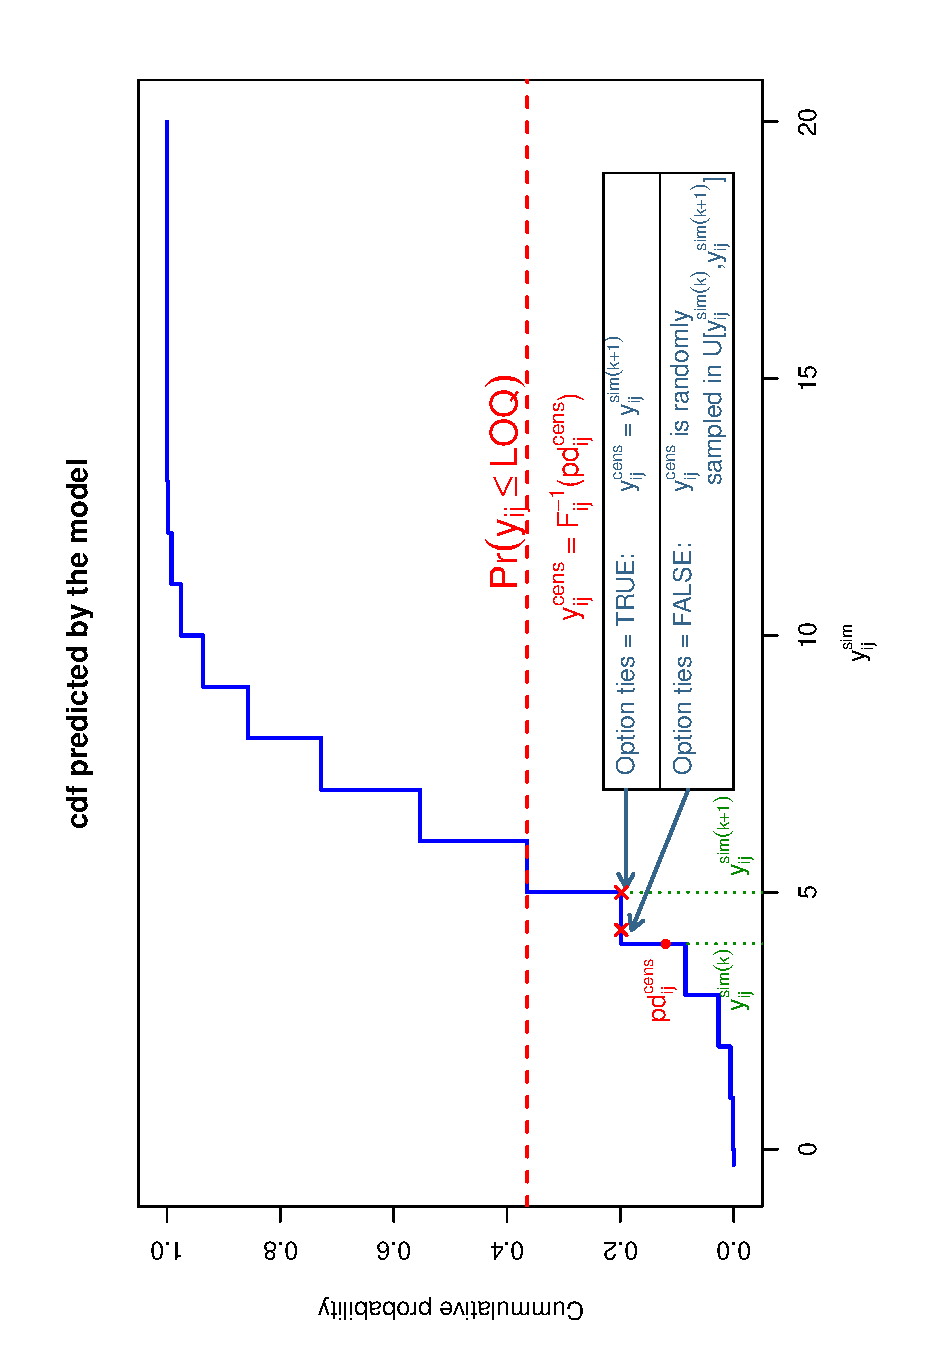
\includegraphics[angle=270,scale=0.7]{/home/eco/work/npde/doclib/figs/imputation.eps}
\caption{Imputation y$_{ij}^{cens}$ from pd$_{ij}^{cens}$ and F$_{ij}$ with the two options {\sf "ties = TRUE"} and {\sf "ties = FALSE"}}
\label{fig:imputation}
\end{figure}

We cannot simply decorrelate the vector of observed data $y_{i}$ using the simulations from the model, because the simulated dataset also contains values that would have been censored and treating them as simulated. We therefore propose to impute these censored data to a value between 0 and LOQ using the same method. We impute a pd$_{ij}^{sim(new),k}$ for each y$_{ij}^{sim,k}$ below LOQ in the simulated data and these y$_{ij}^{sim,k}$ are replaced using the same imputation method applied to the observed data. 
\begin{equation}
y_{ij}^{sim(new),k}=F_{ij}^{-1}(pd_{ij}^{sim(new),k})\,\,\,\mbox{if }y_{ij}^{sim}\leq LOQ
\end{equation}

\bigskip
As previously, to avoid ties in the $\pd$ and $\npde$, we can jitter the imputed $\pd$ and $y$. Figure~\ref{fig:imputation} shows an illustration for both cases:
\begin{itemize}
\item method {\sf "ties = TRUE"}: if $F_{ij}(y_{ij}^{sim(k)}) < pd_{ij}^{cens}\leq F_{ij}(y_{ij}^{sim(k+1)})$, then $y_{ij}^{cens} = y_{ij}^{sim(k+1)}$
\item method {\sf "ties = FALSE"}: if $F_{ij}(y_{ij}^{sim(k)}) < pd_{ij}^{cens}\leq F_{ij}(y_{ij}^{sim(k+1)})$, then $y_{ij}^{cens}$ is randomly sampled in a uniform distribution over the interval [$y_{ij}^{sim(k)},y_{ij}^{sim(k+1)})$]
\end{itemize}

After the imputation step, a new vector of observations Y$_{i}^{new}$ and new simulated data Y$_{i}^{sim_{new}}$ are obtained. The complete data are then decorrelated using the same technique as described above. Note that the matrix $\var(\Y_i)$ used to decorrelate is computed using the imputed data, while the predictive distribution functions $F_{ij}$ are computed using the original simulated data before the imputation step.

\subsection{Tests}

\subsubsection{Tests on the distribution of npde} 
\hskip 18pt Under the null hypothesis that model M$^B$ describes adequately the data in the validation dataset, the $\npde$ follow the $\mathcal{N}(0, 1)$ distribution. We report the first three central moments of the distribution of the $\npde$: mean, variance, skewness, as well as the kurtosis, where we define kurtosis as the fourth moment minus 3 so that the kurtosis for $\mathcal{N}(0,1)$ is 0 (sometimes called excess kurtosis). The expected value of these four variables for the expected $\mathcal{N}(0,1)$ are respectively 0, 1, 0 and 0. We also give the standard errors for the mean (SE=$\sigma/\sqrt{N}$) and variance (SE=$\sigma \; \sqrt{2/(N-1)}$).

We use 3 tests to test the assumption that the $\npde$ follow the $\mathcal{N}(0, 1)$ distribution: (i) a Wilcoxon signed rank test, to test whether the mean is significantly different from 0; (ii) a Fisher test for variance, to test whether the variance is significantly different from 1; (iii) a Shapiro-Wilks test, to test whether the distribution is significantly different from a normal distribution. The package also reports a global test, which consists in considering the 3 tests above with a Bonferroni correction~\cite{Brendel10}. The p-value for this global test is then reported as the minimum of the 3 p-values multiplied by 3, the number of simultaneous tests (or 1 if this value is larger than 1)~\cite{Wright}. A graphical code is used in the library to highlight significant results, similar to the code used by other statistical functions in {\sf R} such as {\sf lm} (see example). The normality test is very powerful, especially with large amount of observations. When the test remains significant even 
after model refinement, QQ-plots should be used to assess model adequacy in addition to the 3 statistical tests. This is especially useful in large datasets where the sheer amount of data will lead to reject even reasonable models.

\subsubsection{Tests for covariate models} 

\hskip 18pt In~\cite{Brendel10}, we proposed two approaches to evaluate a model with or without covariates with a validation dataset. 

In the first approach, for continuous covariates we can test for correlations between the covariate and $\npde$, using the Spearman correlation test; for categorical covariates we can use Wilcoxon or Kruskal-Wallis tests. If the model and validation data correspond, there should be no relationship between $\npde$ and covariates.

In the second approach, we proposed to split the $\npde$ according to the values of the covariate, and test within each category that $\npde$ follows a $\mathcal{N}(0,1)$ distribution. For categorical covariates, $\npde$ are split by categories of the covariate. We proposed to discretise continuous covariates in 3 classes, below first quartile ($<$Q$_1$), between first and third quartiles (Q$_1$--Q$_3$) and above third quartile ($>$Q$_3$). If the model and validation data correspond, there should be no significant departure from $\mathcal{N}(0,1)$ within each category: a test is performed for each category, and the resulting p-values are corrected with a Bonferroni correction.

Both approaches gave similar results in terms of type I error in a simulation study, but the second approach has a slightly larger type I error and a correspondingly slight increase in power~\cite{Brendel10}. Tests for covariate models will be added shortly to the library.

\subsection{Graphs} \label{sec:graphmethods}

\subsubsection{Diagnostic graphs} 

\paragraph{Assessing the distribution of npde:} Graphs can be used to visualise the shape of the distribution of the $\npde$. Classical plots include quantile-quantile plots (QQ-plots) of the distribution of the $\npde$ against the theoretical distribution, as well as  histograms and empirical cumulative distributions of the $\npde$ and $\pd$. We also find that scatterplots of the $\npde$ versus the independent variable, the predicted dependent variables, or covariates, can help pinpoint model deficiencies. Some of these graphs are plotted by default (see section~\ref{sec:graphics}). The package computes for each observation the predicted value as the empirical mean over the $k$ simulations of the simulated predicted distribution (denoted $E_k(y^{sim(k)}_{ij})$), which is reported under the name $\ypred$ along with the $\npde$ and/or $\pd$.

In the field of population PK/PD, graphs of residuals versus predictions use the values predicted by the model even when the residuals have been decorrelated, as is the case for both spe and npde here. Comparing metrics to their theoretical distributions can be done through QQ-plots or histograms [10]. Examples of these different graphs will be shown in the next section.

\paragraph{Probability of being under the LOQ:} Finally, when the dataset includes data below the LOQ, a plot of the probability of being BQL can be useful to assess whether the model is able to adequately predict low values, and is available in the \npde~package.

\paragraph{Prediction intervals:} In the current version of the library, prediction bands around selected percentiles, which can be obtained through repeated simulations under the model being tested, can be added to most graphs to highlight departures from predicted values~\cite{Comets10}. Prediction intervals build on the idea of simulating from the model to evaluate whether it can reproduce the observed data. For the VPC, a 95\% prediction interval on a given percentile (eg the median) can be obtained by computing the median for the K simulated datasets and taking the region where 95\% of these K medians lie. This can also be applied to scatterplots of $\npde$ or $\pd$, where for each percentile plotted in the graph we can compute a prediction interval of a given size. By default, 95\% is used in the \npde~package, and each prediction interval is plotted as a coloured area (blue for the 2.5 and 97.5th percentile and pink for the median); the corresponding 2.5th, 50th and 97.5th percentiles of the observed data are plotted as 
lines or points, and should remain within the coloured areas.

A binning algorithm is used for the prediction intervals (the number of bins can be adjusted by the user). Different options are: (1) equal bin sizes on the X-axis; (2) equal bin widths on the X-axis; (3) optimal binning using a clustering algorithm to select the optimal breaks; (4) user-selected breaks. The binning algorithm uses the \texttt{Mclust} library~\cite{Fraley02,Fraley06} for \texttt{R}, which implements model-based clustering with an EM-algorithm to select the optimal number of clusters for the variable on the X-axis of the graph.

\subsubsection{Graphs for covariate models} 

\hskip 18pt Two types of diagnostic graphs are available in the {\sf npde} library for covariates. First, all the graphs can be split according to the values of the covariate, to examine the $\npde$ separately in each group. We use the representation proposed in~\cite{Brendel10} to evaluate covariate models, where $\npde$ are split by category for discrete covariates or by quantiles for continuous covariates (by default, 3 quantiles are used, $<Q1$, interquartile range $Q1-Q3$ over the middle 50\% value of the covariate, and $>Q3$, but the user can select the number of pertinent categories relative to the problem at hand). Prediction bands are also added to those graphs.

A second type of diagnostic is to plot the $\npde$ or $\npd$ versus covariates, to examine the trends. For continuous covariates, a scatterplot of the metrics versus the covariate is provided, while for categorical covariates, we show boxplots for the different categories.

\subsubsection{VPC} 

\hskip 18pt Visual Predictive Check (VPC) are standard diagnostic graphs that are now available also in the {\sf npde} library. In contrast to $\npde$, they do not handle heterogeneity in the design (eg dose regimen) or covariates, so that they are most useful in balanced designs to evaluate models without covariates. However since they are directly obtained from model observations and predictions they illustrate very nicely the shape of the evolution of independent versus dependent variable. VPC are obtained by simulating repeatedly under the model and plotting selected percentiles of the simulated data, comparing them to the same percentiles in the observed data. By default, the VPC produced in the \npde~package correspond to the median and limits of the 95\% prediction interval (eg, the 2.5th, 50th and 97.5th percentile of the data). The observed data can also be plotted over the interval, or omitted for very large datasets.

In the presence of censored data, the same imputation method is also applied to the VPC. For instance, with the default method ({\sf cens.method='cdf'}), the data under the LOQ is set to the value imputed from the predictive distribution through the imputed $\pde$, as described in methods, for {\sf cens.method='ipred'} it it replaced by the corresponding individual predictions (which then have to be given in the dataset), while for {\sf cens.method='omit'}, it is removed from the dataset. In this last case, the simulated data used to compute the prediction bands is also removed from the simulated dataset, yielding larger prediction bands reflecting the lower number of observations involved.

\paragraph{Stratification:} when the model contains covariate effects, traditional VPC should be stratified and examined in each group. Alternatively, corrections such as pcVPC have been proposed, but are not implemented in the {\sf npde} library.

\subsubsection{Graphs with a reference profile}

\hskip 18pt A new feature of the {\sf npde} library is the ability to add a reference plot to the scatterplot of $\npde$ or $\npd$ versus the independent variable. 

% Under the null hypothesis, we expect pde to follow the distribution  $\mathcal{U}[0,1]$ and npde to follow the distribution $\mathcal{N}(0,1)$. It should be noted that left-censored observations in the validation datasets are imputed using the model to be evaluated, which could lead to loss of power if the model is wrong.	


\clearpage
\newpage \section{The npde package} \label{sec:progdesc}

\subsection{Preparation of the input}

\hskip 18pt The library needs two files: 
\begin{itemize} 
\item the file containing the dataset to be evaluated (hereafter named 'observed data') \item the file containing 
the simulations (hereafter named 'simulated data') 
\end{itemize} 
The library does not perform the simulations. {\sf R}, {\sf NONMEM}~\cite{NONMEM}, {\sf 
MONOLIX}~\cite{Monolix} or any program of your choice can be used for that purpose.

\subsubsection{Observed data}

\hskip 18pt The observed data file must contain at least the following 3 columns: 
\begin{itemize} 
\item id: patient identification 
\item xobs: independent variable (time, X, ...) 
\item yobs: dependent variable (DV, concentrations, 
effects...) 
\end{itemize} 
Additional (optional) columns may be given. The program will recognise the following 
input: 
\begin{itemize} 
\item cens: censoring information (0 for observed data, 1 for censored data) 
\item mdv: missing data (0 for observed data, 1 for missing data); this information supersedes censoring 
information, so that an observation with mdv equal to 1 will be treated as missing, not as censored; observations 
with values "." or NA will also be considered as missing 
\item ipred: individual model predictions 
\item covariates 
\end{itemize} 
The computation of \pd~and \npde~will remove missing observations from the observed dataset reported in the output 
(see section~\ref{sec:results}). If other names than {\sf cens} and {\sf mdv} are used in the original dataset, 
they will be renamed to {\sf cens} and {\sf mdv} in the {\sf data} slot of the object.

Other columns may be present but will not be used by the library. The actual order of the columns is unimportant, 
since the user may specify which column contain the requested information, but the default order is 1. id, 2. xobs, 
3. yobs and no MDV column. A file header may be present, and column separators should be one of: blank space(s), 
tabulation mark, comma (,) or semi-colon (;). Finally, the digit mark should be a dot as in English (eg a number 
would read 4.5) and not a comma as in French (4,5).

\subsubsection{Simulated data}

\hskip 18pt The user must provide a file containing the K simulated datasets stacked one after the other. Within 
each simulated dataset, the order of the observations must be the same as within the observed dataset. The 
dimensions of the two datasets must be compatible: if n$_{\rm obs}$ is the number of lines in the observed dataset, 
the file containing the simulated datasets must have K$\times$n$_{\rm obs}$ lines.

The simulated data file must contain at least 3 columns, in the following order: \begin{enumerate} \item id : 
patient identification \item xsim: independent variable (time, X, ...) \item ysim: dependent variable (DV, 
concentrations, effects...) \end{enumerate} Additional columns may be present but will not be used by the library.

The length of the \textcolor{violet}{id} (resp \textcolor{violet}{xobs}) column must be equal to the length of the 
\textcolor{violet}{id} (resp \textcolor{violet}{xobs}) column of the observed dataset repeated K times.

An example of how to set up simulations for an example dataset can be found in section~\ref{sec:exampletheo}, and 
examples of a simulated and observed dataset are available in the subdirectory {\sf doc/inst} of the library.

\subsubsection{Number of simulations}

\hskip 18pt Based on the results of simulation studies~\cite{Brendel10,Comets10}, we recommend to use at least 
$K$=1000 but the actual number may depend on the dataset involved, and should be increased when the dataset 
includes a large number of subjects. This will be investigated in more details in future work on {\sf npde}. A 
warning will be issued when $K$ is smaller than 1000 (see examples in section~\ref{sec:npde.examples}).

\subsection{Execution}

\subsubsection{Interactive execution}

\hskip 18pt The interactive mode is called by the function {\sf npde()}: 
\begin{verbatim} 
myres<-npde() 
\end{verbatim} 
The user will be prompted to enter successively: 
\begin{itemize} \item the name of the file or dataframe containing the observed data 
\item the columns in which id, xobs, dependent variable yobs, and possibly 
column with missing data MDV can be found (the default order is 1, 2, 3 and no MDV column) \item the name of the 
file or dataframe containing the simulated data 
\item whether results should be saved to disk; if so, the user must also enter 
    \begin{itemize} 
    \item the format of the graph (one of: Postscript, JPEG, PNG or PDF) 
    \item the name of the files: an extension {\sf .npde} will be added to this name for the file in which 
numerical     results are to be saved (see section~\ref{sec:results}), and an extension depending on the format of 
the graph will     be added to this name for the file in which graphs are to be saved (respectively .eps, .jpeg, 
.png, .pdf for the     formats above). For instance, if the user enters {\sf myoutput} and requests that the graphs 
be saved in PDF     format, the results file will be named {\sf myoutput.npde} and the graph files will be {\sf 
myoutput.pdf}. 
    \end{itemize} 
\item whether $\npde$ should be computed \item whether $\pd$ should be computed \item whether a message should be 
printed as the computation of $\npde$ begins in a new subject 
\item whether the function should return values (see section~\ref{sec:value}) 
\end{itemize} 
Alternatively, one or both filenames for the observed and simulated data 
can be replaced by a dataframe if the data has already been loaded in {\sf R} (see example in the online 
documentation provided with the package).

\subsubsection{Non-interactive execution}

\hskip 18pt In the non-interactive mode, the required information is fed to the function {\sf autonpde()} instead 
of answering a series of questions. The minimum input should include the name of the observed data file (for 
example, {\sf theopp.tab}) and the name of the simulated data file (for example, {\sf simtheopp.tab}), as in: 
\begin{verbatim} autonpde("theopp.tab","simtheopp.tab") \end{verbatim} A number of options can also be set as 
arguments, and are given in table~I. \begin{table}[!h] \noindent{\bfseries Table I:} {\itshape Options available 
for the autonpde function.} \begin{center} \begin{tabular} {l p{8cm} c} \hline \textbf{Option} & \textbf{Effect} & 
\textbf{Default value} \\ \hline iid & number of the column with ID information in the observed data file & 1 \\ ix 
& number of the column with the independent variable (X) & 2 \\ iy & number of the column with the observed data 
(Y) & 3 \\ imdv & number of the column indicating missing data (MDV) & 0 \\ icens & number of the column indicating 
censoring (CENS) & 0 \\ iipred & number of the column with individual predictions (IPRED) & 0 \\ detect & if TRUE, 
the datafile containing the original data is assumed to have a header, and the program will attempt to guess which 
columns contain ID, X, Y, MDV, CENS and IPRED & FALSE \\ units & units for the X and Y axis (will be used in plots) 
& none \\ boolsave & whether results should be saved to disk & TRUE \\ namsav & name of the files where results 
will be saved (without extension) & output\\ type.graph & graph format (one of: Postscript, JPEG, PNG or PDF, 
corresponding to extensions .eps, .jpeg, .png and .pdf respectively for the graph file) & eps \\ calc.npde & 
whether normalised prediction distribution errors should be computed &  TRUE \\ calc.pd & whether prediction 
discrepancies should be computed & TRUE \\ decorr.method & method used to decorrelate & cholesky \\ cens.method & 
method used to handle censored data & impute \\ ties & if FALSE, the distributions of \pd and \npde are smoothed to 
avoid ties & TRUE \\ verbose & whether a message should be printed as the computation of $\npde$ begins in a new 
subject &  FALSE \\ \hline \end{tabular} \end{center} \end{table} Note that option \texttt{output} has been 
deprecated (the \texttt{invisible()} option is used to suppress the output when it is not affected to an object).

\bigskip Here is an example of the call to {\sf autonpde()} with a number of arguments (see example in 
section~\ref{sec:expde} for an illustration): \begin{verbatim} 
x<-autonpde(namobs="theopp.tab",namsim="simtheopp.tab",iid=1,ix=2,iy=3, 
imdv=0,namsav="output.eps",boolsave=T,type.graph="eps",output=F,verbose=T) \end{verbatim}

\clearpage \subsection{Results} \label{sec:results}

\hskip 18pt Both execution modes will produce the same results. Three types of results are produced by default, but 
options can be used so that only some of them are created: \begin{enumerate} \item an {\sf R} object of class 
NpdeObject, containing several elements, including the $\npde$ and/or $\pd$ (see section~\ref{sec:value}). With the 
option {\sf output=F} the object is not returned. \item a graph file containing diagnostic plots of the $\npde$ 
({\sf output.eps} with the default values; see section~\ref{sec:graphics}). The graph also appears in the graphic 
window of the current {\sf R} session. With the option {\sf boolsave=F} the graph is shown but not saved to a file. 
\item a text file with the same name as the graph file and extension {\sf .npde} containing the following data 
({\sf output.npde} with the default values), organised in columns: id, xobs, ypred, npde, pd With the option {\sf 
boolsave=F}, the results are not saved. \end{enumerate}

\subsubsection{Value}~\label{sec:value}

\hskip 18pt By default, the function returns an object of class NpdeObject: \begin{verbatim} myres<-npde() 
\end{verbatim} Version 2.0 of the \npde~package uses the S4 class system, and many functions have been defined to 
handle the object and produce descriptive summaries and plots (please refer to section~\ref{sec:npde.methods} for 
more details about S4 classes). As a result, the output is no longer a list that can be manipulated, but a slightly 
more complicated object. However, for compatibility with the previous version of \npde, a \texttt{summary} function 
can be used to produce a list containing the main results: \begin{verbatim} x1<-summary(myres) \end{verbatim}

\bigskip The object returned by the function contains 5 elements: \begin{enumerate} \item \textbf{data}: a NpdeData 
object containing the information relative to the observed data \item \textbf{datsim}: a NpdeSimData object 
containing the information relative to the simulated data \item \textbf{results}: a NpdeRes object containing the 
results \item \textbf{options}: a list of options used in the computations \item \textbf{prefs}: a list of 
graphical preferences \end{enumerate} The first three elements are S4 objects also, with their own class and own 
methods, while the last two elements are R lists. More information on how to handle these objects and which methods 
have been defined for them can be found in~\ref{sec:npde.methods}.

\subsubsection{Graphs} \label{sec:graphics}

\hskip 18pt Four graphs are produced by default: \begin{enumerate} \item a quantile-quantile plot: plot of the 
$\npde$ versus the corresponding quantiles of a normal distribution \begin{itemize} \item the line $y=x$ is also 
drawn \end{itemize} \item a histogram of the $\npde$ \begin{itemize} \item the shape of the normal distribution 
$\mathcal{N}(0,1)$ is also shown \end{itemize} \item a plot of the $\npde$ versus the independent variable X \item 
a plot of the $\npde$ versus ypred \begin{itemize} \item for these last two graphs, we plot the lines corresponding 
to $y=0$ and to the critical values 5\% and 95\% (delimiting the 90\% confidence interval in which we expect to 
find the bulk of the $\npde$). \end{itemize}   \end{enumerate} The default graphs now include (approximated) 
prediction intervals (obtained by simulating from the theoretical $\mathcal{N}(0,1)$ distribution, see 
section~\ref{sec:graphmethods}); for compatibility with the behaviour of \npde~version 1.2, the option {\sf 
bands=FALSE} can be used to suppress plotting the prediction intervals.

These graphs are designed as diagnostics for the $\npde$; a function providing similar graphs for $\pd$ is {\sf 
plotpd}.

\subsection{Errors during execution}

\hskip 18pt Sometimes the function is unable to compute the decorrelated prediction distribution errors for one or 
more subjects. The following error messages can appear: \begin{verbatim} The computation of the npde has failed for 
subject xx because the Cholesky decomposition of the covariance matrix of the simulated data could not be obtained. 
\end{verbatim} or \begin{verbatim} The computation of the npde has failed for subject xx because the covariance 
matrix of the simulated data could not be inverted. \end{verbatim} followed by: \begin{verbatim} This usually means 
that the covariance matrix is not positive-definite. This can be caused by simulations widely different from 
observations (in other words, a poor model). We suggest to plot a prediction interval from the simulated data to 
check whether the simulations are reasonable, and to consider prediction discrepancies. Prediction discrepancies 
will now be computed. \end{verbatim} In our experience, this usually happens when the model is so ill-conditioned 
that the matrices involved in the computation of the prediction distribution errors are singular, and mostly 
happens when the model predicts the data very poorly. A prediction interval (or Visual Predictive Check) can be 
plotted to check this.

When $\npde$ cannot be computed, the program computes automatically $\pd$ even if the {\sf calc.pd=F} option was 
used. The following graphs are plotted using $\pd$ instead of $\npde$ \begin{enumerate} \item a quantile-quantile 
plot: plot of the $\pd$ versus the corresponding quantiles of a uniform distribution \begin{itemize} \item the line 
$y=x$ is also drawn \end{itemize} \item a histogram of the $\pd$ with the uniform density $\mathcal{U}(0,1)$ 
overlain \item a plot of the $\pd$ versus the independent variable X \item a plot of the $\pd$ versus $\ypred$ 
\begin{itemize} \item for these last two graphs, we plot the lines corresponding to $y=0$ and to the 5\% and 95\% 
critical values (delimiting the 90\% confidence interval in which we expect to find the bulk of the $\pd$). 
\end{itemize} \end{enumerate} In this case, approximated prediction intervals are not plotted by default, since the 
approximation (sampling from the standard gaussian distribution) neglects the correlation between the different 
$\pd$ in an individual, and this leads to substantially narrower prediction intervals when the number of data per 
subject is large. Prediction bands may be added by combining the option {\sf bands=TRUE} with option {\sf 
approx.pi} set to either \texttt{TRUE} for an approximated prediction interval (fast but rough) or \texttt{FALSE} 
for an approximated prediction interval (obtained using the simulated datasets), as in: \begin{verbatim} 
x<-dist.pred.sim(x) plot(x,bands=TRUE,approx.pi=TRUE) \end{verbatim} As seen here, requesting an exact (simulated) 
prediction interval requires first to compute the distribution of $\pd$ in the simulated dataset, using the 
function \texttt{dist.pred.sim} (by default and in the interest of time, this function computes only the 
distribution of the $\pd$, but if called with the additional argument {\sf calc.npde=TRUE} the $\npde$ in the 
simulated dataset will also be included in the output, allowing the user to use \texttt{approx.pi=TRUE} for graphs 
including $\npde$).

\subsection{Functions in the \npde~package} \label{sec:npde.methods}

\hskip 18pt \npde~has been programmed using the S4 classes in \R. S4 classes implement Object oriented programming 
(OOP) in \R, allowing to construct modular pieces of code which can be used as black boxes for large systems. Most 
packages in the base library and many contributed packages use the former class system, called S3. However, S4 
classes are a more traditional and complete object oriented system including type checking and multiple 
dispatching. S4 is implemented in the methods package in base \R. More information on S4 classes and \R packages 
can be found in tutorials on the Web. I used extensively the following manual~\cite{Genolini} (in French).

The object returned by the \texttt{npde()} and \texttt{autonpde()} functions has the \texttt{NpdeObject} class, and 
both generic and specific methods have been defined for this class: \begin{itemize} \item print: the print function 
produces a summary of the object in a nice format \item show: this function is used invisibly by \R when the name 
of the object is typed, and produces a short summary of the object (more details can be obtained by using the 
alternative \texttt{showall()} function \item summary: this function produces a summary of the object, and 
invisibly returns a list with a number of elements, which provides an alternative way to access elements of the 
class; the list contains the following elements: \begin{itemize} \item[obsdat] the data (a matrix with 3 columns, 
id=subject id, xobs=observed X, yobs=observed Y, plus if present in the data additional columns containing censored 
information, mdv, covariates, ...) \item[id] subject id (first column in obsdat) \item[x] observed x (second column 
in obsdat) \item[y] observed y (third column in obsdat) \item[npde] the computed $\npde$ \item[pd] the computed 
prediction discrepancies \item[ploq] the probability of being BQL for each observation (if computed) \item[N] 
number of subjects \item[nrep] number of simulations used in the computations \item[ntot.obs] total number of 
non-missing observations \item[ypred] predicted Y (the empirical mean of the simulated predicted distribution for 
each observation ($E_k(y^{sim(k)}_{ij})$)) \item[ycomp] completed vector of observed y (includes the values that 
were imputed during the computation when BQL data are in the dataset) \item[ydobs] the decorrelated observed data 
$y_{ij}^*$ \item[ydsim] the decorrelated simulated data $y^{sim(k)*}_{ij}$ \item[xerr] an integer valued 0 if no 
error occurred during the computation or a positive number (1 or 2) depending on the error encountered, if an error 
occurred \item[options] options (can also be seen by using the \texttt{print} function) \item[prefs] graphical 
preferences (can also be seen by using the \texttt{print} function) \end{itemize} \item plot: this produces plots 
of the different objects \begin{itemize} \item when called without any argument, the default four plots are 
produced \item an argument plot.type can be used to produce different plots \item all plots can be tweaked to add 
titles, change colours,... \end{itemize} \item $[$ function: the get function, used to access the value of the 
slots in an object \item $[<$-: function: the set function, used to replace the value of the slots in an object 
\item gof.test: goodness-of-fit tests on the distribution of \texttt{npde} (or \texttt{pd}) \end{itemize} Examples 
of calls to these functions are given in the corresponding man pages and in the documentation 
(section~\ref{sec:exampletheo}).

\subsection{Options for graphs}

\hskip 18pt The document \verb+ test_npde.pdf+ has been created to test the \npde~library and showcase the 
different graphs. It contains several fits for the datasets shown in section~\ref{sec:npde.examples}, and provides 
many examples of graphs setting graphical options. There is also a list of the graphical options with their 
significance. This document is included in the \verb+inst+ directory, where the present guide is also located.

\bigskip An object \texttt{x} resulting from a call to {\sf npde()} or {\sf autonpde()} contains a slot 
\texttt{prefs} where the graphical preferences are stored as a list. Options can be set on the fly for a given 
plot, by simply adding them to the call to {\sf plot()} as an argument (see examples in 
section~\ref{sec:npde.examples}), and they will then supersede the preferences attached to the object: 
\begin{verbatim} plot(x,plot.type="data",col="red",main="Raw data") \end{verbatim} The options can also be modified 
directly in the object, and they will then apply to the next plots, for instance changing the new default color to 
red for all plots is done by setting the attribute {\sf col} in the list: \begin{verbatim} x["prefs"]$col<-"red" 
\end{verbatim} Options given on the fly will always supersede the options stored in the \texttt{prefs} slot.

\paragraph{Binning:} most graphs now have the option of added prediction intervals. These prediction intervals are 
computed using simulations under the model, and they require a binning algorithm. The influence of the number and 
position of bins is quite important for the visual assessment of the fit.

Several options are available for binning, and can be set using the \texttt{vpc.method} option. Possible options 
are: \begin{itemize} \item \texttt{equal}: uses quantiles of the data to have about the same number of points in 
each bin \item \texttt{width}: divides the interval into bins of equal size \item \texttt{user}: user-defined 
breakpoints, set in \texttt{vpc.breaks} (will automatically be expanded to include the lower and upper value of the 
data if not provided) (if \texttt{vpc.breaks} is not supplied, the \texttt{equal} method will be used instead) 
\item \texttt{optimal}: uses the \texttt{Mclust} function from the \texttt{mclust} library (when available) to 
provide the optimal clustering; the Mclust method \end{itemize} With all methods, if the number of bins requested 
is larger than the number of unique values of X, the number of bins will be limited to the number of unique values.

\begin{description} 
\item[Warning:] when using the 'optimal' method, warnings may appear. The optimal number of bins is selected from 
a range equal to \texttt{vpc.bin} $\pm 5$, but a message such as:
'\verb+In map(out$z) : no assignment to 2,4,8,11+' usually indicates that the number of bins is too large, it is 
then advised to change the value of \texttt{vpc.bin} and start again. 
\end{description}

Specifying c(0.01,0.99) with the '\texttt{equal}' or '\texttt{width}' binning method and vpc.bin=10 will create 2 
extreme bands containing 1\% of the data on the X-interval, then divide the region within the two bands into the 
remaining 8 intervals each containing the same number of data; in this case the intervals will all be equal except 
for the two extreme intervals, the size of which is fixed by the user; complete fine-tuning can be obtained by 
setting the breaks with the vpc.method="user"

\paragraph{Further options:} More details on available graphs and options can be found in the online documentation. 
Please type: 
\begin{verbatim} 
?plot.npde 
\end{verbatim} to get started. 
% The npde library contains 14 functions. Figure~\ref{fig:functionhierar} presents 
% the functions hierarchy starting with function {\sf npde}. A similar graph is 
% obtained with function {\sf autonpde} without the call to function {\sf % pdemenu}. 
% \begin{figure}[!h] %\begin{center} 
% 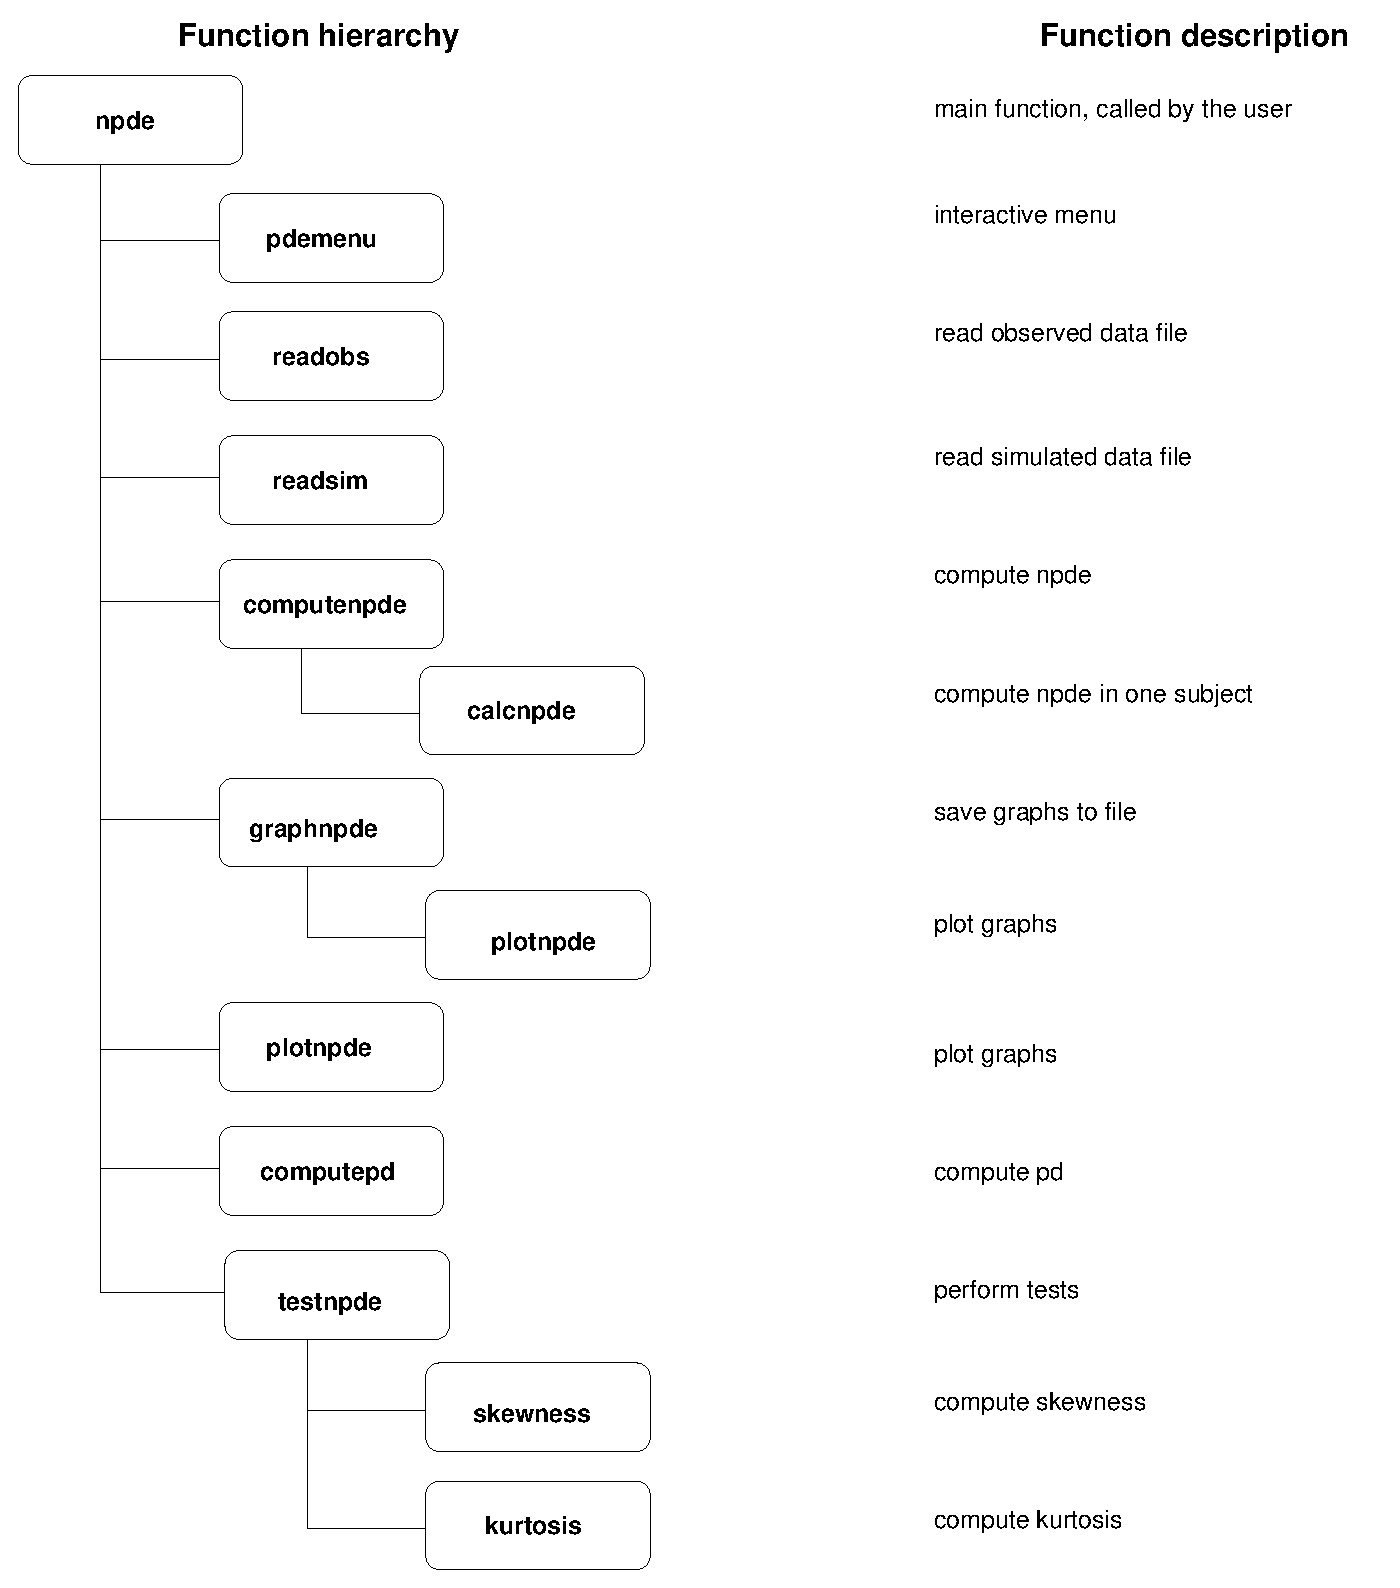
\epsfig{file=/home/eco/work/npde/doclib/figs/hierarchyhelv.eps,width=16cm,angle=0} % \end{center} 
% \par \kern -1cm 
% \caption{Function hierarchy for the npde package, and brief description of each 
% function. The functional hierarchy is given for a user call to npde. With 
% autonpde, the hierarchy is the same save for the initial call to pdemenu.} 
% \label{fig:functionhierar} 
% \end{figure}

If further tweaking is required, any graph can also be recreated with a bit of work using the output from the 
package. Using the function \texttt{summary} will extract the necessary elements from the object, and the user can 
then use those to produce her or his own graphs. \begin{verbatim} x1<-summary(x) names(x1) head(x1$x) head(x1$npde) 
\end{verbatim}

\clearpage \newpage


\clearpage
\section{Examples} \label{sec:npde.examples}

\subsection{Model evaluation for theophylline PK} \label{sec:exampletheo}

\hskip 18pt The subdirectory {\sf doc} contains a full working example using {\sf npde}. We used the {\sf theopp.tab} dataset provided with {\sf NONMEM} as an example which most users are already familiar with. This dataset is also available under the name {\sf Theoph} in the {\sf dataset} package in {\sf R}, under a slightly different format. This dataset was provided by a study by Dr. Robert Upton of the kinetics of the anti-asthmatic drug theophylline~\cite{NONMEM}.

The subdirectory {\sf doc} contains the following files:
\begin{center}
\begin{tabular} {l l}
\hline
theopp.tab & the observed data \\
simtheopp.tab & the simulated data (with $K$=100)$^1$ \\
fittheop.ctr & the NONMEM control file used for the estimation\\
simultheop.ctr & the NONMEM control file used for the simulations\\
runtheo.res & the result file from the NONMEM estimation \\
theophylline.eps & the graphs \\
theophylline.npde & the file containing the results \\
npde\_userguide.pdf & the present user guide \\
vtrue.dat$^2$ & a file with data simulated under H$_0$ \\
vfalse.dat$^2$ & a file with data simulated assuming a bioavailability divided by 2\\
\hline
\end{tabular}
\end{center}
\noindent$^1$ {\itshape We used K=100 to provide a very quick computation of the $\npde$ and to avoid including a large file in the package, however we recommend using at least K=1000 for the simulations.}

\noindent$^2$ {\itshape These datasets were simulated as examples of external validation datasets in~\cite{CometsCMPB08}}

%\newpage
\subsubsection{Data}

\hskip 18pt Theophylline concentrations were measured in 12 patients over a period of 24~hr after a single oral dose of the drug. Each patient received a different dose. The data file has the following structure:
\begin{center}
\begin{tabular} {l c c c c c}
\hline
Column number & 1 & 2 & 3 & 4 & 5 \\
Column name & ID & Dose & Time & Conc & Wt \\
Item meaning & Patient id & Dose & Time & Concentrations & Weight \\
\hline
\end{tabular}
\end{center}
Doses are given in~mg, times in hours and concentrations are reported in mg.L$^{-1}$.

Figure~\ref{fig:theodata} displays the dataset. The data for the first two patients is given in the appendix (see page~\pageref{sec:appdata}), to show the format of the data file.
\begin{figure}[!h]
\par\kern -0.3cm
\begin{center}
\epsfig{file=/home/eco/work/npde/npde30/latexDoc/figsDev/doc_theodata_gg.eps,width=13cm}
\end{center}
\caption{Theophylline data.}\label{fig:theodata}
\end{figure}

\subsubsection{Model}

\hskip 18pt The data was analysed with a one-compartment model with first-order absorption and elimination, parameterised in absorption rate constant k$_a$ (units hr$^{-1}$) volume of distribution V (units L) and elimination rate constant k (units hr$^{-1}$). Concentrations at time 0 were removed from the dataset. The model did not include covariates. Interindividual variability was modelled using an exponential model for the three pharmacokinetic parameters. A covariance between the parameters k and V was assumed, yielding the following variance-covariance matrix:
\begin{equation}
\Omega=\left(
\begin{array}{ccc}
\omega_{k_a}^2 & 0 & 0\\
0 & \omega_{V}^2 & omega_{k,V}={\rm cov}(\eta_{k},\eta_{V}) \\
0 & {\rm cov}(\eta_{k},\eta_{V}) & \omega_{k}^2\\
\end{array}
\right)
\end{equation}
The residual error model was a combined additive and proportional
error model as in equation~\ref{eq:errormod}.

\bigskip These data were analysed with the software {\sf NONMEM} version 5.1. The ADVAN2 routine was used. The estimation method was the {\sf FOCE} algorithm with the {\sf INTERACTION} option. The control file is given in the Appendix (see page~\pageref{sec:appanalctr}) and the relevant results in the ouput file {\sf runtheo.res} are shown on page~\pageref{sec:appresnonmem}.

The following parameter estimates were obtained:
\begin{center}
\begin{tabular} {l c | l c}
\hline 
\multicolumn{2}{c}{Population mean} & \multicolumn{2}{c}{Interindividual
variability (CV\%)} \\
\hline 
k$_a$ (hr$^{-1}$) & 1.51 & $\omega_{k_a}$ (-) & 0.67 \\
V (L) & 0.46 & $\omega_{V}$ (-) & 0.12 \\
k (L.hr$^{-1}$) & 0.087 & $\omega_{k}$ (-) & 0.13 \\
$\sigma_{\rm inter}$ (mg.L$^{-1}$) & 0.088 & cor$(\eta_{k},\eta_{V})$ (-) & 0.99 \\
$\sigma_{\rm slope}$ (-) & 0.26 & &\\
\hline
\end{tabular}
\end{center}

\subsubsection{Simulations}

\hskip 18pt The simulations were also performed using {\sf NONMEM} version 5.1. The control file used for the simulations is given in the Appendix (see page~\pageref{sec:appsimulctr}). The beginning is identical to the control file used for the analysis (page~\pageref{sec:appresnonmem}); the initial values in the {\sf \$THETA}, {\sf \$OMEGA}, {\sf \$SIGMA} blocks have been changed to the values estimated with the model, the {\sf \$ERROR} block includes a line to output the simulated data, and the {\sf \$TABLE} block has been changed to output the simulated data in a file.

The number of simulations can be changed with the {\sf SUBPROBLEMS} options in the {\sf \$SIMULATION} block. Here, we use 100 simulations to compute the $\npde$ quickly as an illustration, but larger numbers are more appropriate (we recommend at least 1000 simulations). Simulations were saved in the file {\sf simtheopp.tab}.

\subsubsection{Computing $\npde$} \label{sec:expde}

\hskip 18pt The interactive version of the program was run below. In a first step, the user was prompted to enter all details necessary for the computations (text \textcolor{mycol}{\bf in purple} show values entered by the user while text in black is printed by the program):

\bigskip
{\sf
\noindent myres<-npde() \\
Name of the file containing the observed data: \textcolor{mycol}{\bf theopp.tab}\\
Automatic recognition of columns in the dataset (y/Y) [default=yes] ? \textcolor{mycol}{\bf n}\\
I'm assuming file theopp.tab has the following structure:\\
$\phantom{me}$\hskip 0.5cm        ID X Y ...\\
and does not contain a column signaling missing data.\\
To keep, press ENTER, to change, type any letter: \textcolor{mycol}{\bf n}\\
$\phantom{me}$\hskip 0.5cm Column with ID information ? \textcolor{mycol}{\bf 1}\\
$\phantom{me}$\hskip 0.5cm Column with X (eg time) information ? \textcolor{mycol}{\bf 3}\\
$\phantom{me}$\hskip 0.5cm Column with Y (eg DV) information ? \textcolor{mycol}{\bf 4}\\
$\phantom{me}$\hskip 0.5cm Column signaling missing data (eg MDV, press ENTER if none) ? \\
$\phantom{me}$\hskip 0.5cm Column signaling censoring (eg CENS, press ENTER if none) ? \\
$\phantom{me}$\hskip 0.5cm Column with individual predictions (eg ipred, press ENTER if none) ?  \\
$\phantom{me}$\hskip 0.5cm Columns with covariates (eg WT; enter one at a time, press ENTER if none or when finished) ?  \\
Name of the file containing the simulated data: \textcolor{mycol}{\bf 
simtheopp.tab}\\
Do you want results and graphs to be saved to files (y/Y) [default=yes] ? \textcolor{mycol}{\bf y}\\
Different formats of graphs are possible:\\
$\phantom{me}$\hskip 0.5cm         1. Postscript (extension eps)\\
$\phantom{me}$\hskip 0.5cm         2. JPEG (extension jpeg)\\
$\phantom{me}$\hskip 0.5cm         3. PNG (extension png)\\
$\phantom{me}$\hskip 0.5cm         4. Acrobat PDF (extension pdf)\\
Which format would you like for the graph (1-4) ? \textcolor{mycol}{\bf 1}\\
Name of the file (extension will be added, default=output): 
\textcolor{mycol}{\bf theophylline}\\
Do you want to compute npde (y/Y) [default=yes] ? \textcolor{mycol}{\bf y}\\
Do you want to compute pd (y/Y) [default=yes] ? \textcolor{mycol}{\bf y}\\
Different decorrelation methods are available:\\
$\phantom{me}$\hskip 0.5cm         1. Cholesky decomposition (default)\\
$\phantom{me}$\hskip 0.5cm         2. Inverse using diagonalisation (as in Monolix and Nonmem)\\
$\phantom{me}$\hskip 0.5cm         3. Cholesky followed by polar decomposition\\
Which method should be used for the decorrelation (1-3) ? \textcolor{mycol}{\bf 1}\\
Method used to handle censored observations:\\
$\phantom{me}$\hskip 0.5cm         1. omit: pd will be set to NaN for missing data\\
$\phantom{me}$\hskip 0.5cm         2. cdf: pd will be imputed using a random sample from U(0,p\_LOQ) where p\_LOQ is the probability, according to the model, that a given observation is less than LOQ (default)\\
$\phantom{me}$\hskip 0.5cm         3. loq: an observation below the LOQ will be imputed to the LOQ\\
$\phantom{me}$\hskip 0.5cm         4. ypred: an observation below the LOQ will be imputed to the population model prediction\\
$\phantom{me}$\hskip 0.5cm         5. ipred: an observation below the LOQ will be imputed to the individual model prediction\\
Which method should be used (1-5) ? \textcolor{mycol}{\bf 2}\\
Do you want a message printed as the computation of npde begins in a new
subject (y/Y) [default=no] ? \textcolor{mycol}{\bf y}\\
Do you want the function to return an object (y/Y) [default=yes] ? \textcolor{mycol}{\bf y}\\
}

In the second step, the program computed the normalised prediction distribution errors, plotted the corresponding graphs and performed the statistical tests for $\npde$, then computed the prediction discrepancies (for which no tests are reported). A warning is issued here because the number of simulations is considered too small. 

Here we see that the test of the mean (\texttt{t-test}) and variance (\texttt{Fisher variance test}) don't shown any significant departure from the theoretical values of 0 and 1 respectively, on the other hand, the normality test (\texttt{SW test of normality}) indicates a departure from the normal distribution, so that the global test (\texttt{Global adjusted p-value}), consisting of a Bonferroni-corrected combination of the three test, also shows a significant departure from the theoretical distribution. However, the results of the tests don't necessarily reflect model adequacy in this case, because of the small number of simulations used.
%\newpage
{\small
\begin{verbatim}
Automatic detection of variables is ON. The program will attempt to detect
both mandatory variables (ID, X, Y) and optional variables (IPRED, MDV, CENS) 
when they are not specifically given or when the user-specified names are not 
found in the dataset, by looking in the names of the columns (to override this 
behaviour, please use argument detect=FALSE in the call to npdeData().
Reading data from file ../data/theopp.tab 
These are the first lines of the dataset as read into R. Please check the format 
of the data is appropriate, if not, modify the na and/or sep items and retry:
  ID Dose Time  Conc   Wt
1  1 4.02 0.00    NA 79.6
2  1   NA 0.25  2.84   NA
3  1   NA 0.57  6.57   NA
4  1   NA 1.12 10.50   NA
5  1   NA 2.02  9.66   NA
6  1   NA 3.82  8.58   NA

The following NpdeData object was successfully created:
Object of class NpdeData
    longitudinal data
Dataset ../data/theopp.tab 
    Structured data: Conc ~ Time | ID 
    predictor: Time (hr) 
NpdeDataReading data from file ../data/simtheopp.tab 
These are the first lines of the dataset as read into R. Please check the format 
of the data is appropriate, if not, modify the na and/or sep items and retry:
  ID xsim      ysim
1  1 0.00 -0.090212
2  1 0.25  2.289200
3  1 0.57  4.227900
4  1 1.12  5.497900
5  1 2.02  7.917300
6  1 3.82  5.394300
There are rows with MDV=1 in the original dataset, the corresponding rows 
will be removed from the simulated dataset.

Warning: the number of simulations is 100 which may be too small.
We advise performing at least 1000 simulations to compute npde.
Computing the npde for subject  1 
Computing the npde for subject  2 
Computing the npde for subject  3 
Computing the npde for subject  4 
Computing the npde for subject  5 
Computing the npde for subject  6 
Computing the npde for subject  7 
Computing the npde for subject  8 
Computing the npde for subject  9 
Computing the npde for subject  10 
Computing the npde for subject  11 
Computing the npde for subject  12 

---------------------------------------------
Distribution of npde :
      nb of obs: 120 
           mean= 0.0668   (SE= 0.095 )
       variance= 1.074   (SE= 0.14 )
       skewness= 0.511 
       kurtosis= 0.2912 
---------------------------------------------

Statistical tests (adjusted p-values):
  t-test                : 1
  Fisher variance test  : 1
  SW test of normality  : 0.00819 **
  Global test           : 0.00819 **
---
Signif. codes: '***' 0.001 '**' 0.01 '*' 0.05 '.' 0.1 
---------------------------------------------
\end{verbatim}
}

\paragraph{Note:} the p-values are now all presented after adjustement with a Bonferroni correction. In the previous versions of {\sf npde} only the global test was adjusted, while the other p-values were presented as raw values. We have now changed this for consistency.

%\begin{verbatim}
% Previously... why changed ??? (including mean & moments => check computation)
% Saving graphs in file keepnpde/inst/doc/theophylline.eps 
% ---------------------------------------------
% Distribution of npde:
%            mean= 0.05641   (SE= 0.092 )
%        variance= 1.024   (SE= 0.13 )
%        skewness= 0.4065 
%        kurtosis= 0.0888 
% ---------------------------------------------
% 
% Statistical tests
%   Wilcoxon signed rank test  : 0.883
%   Fisher variance test       : 0.823
%   SW test of normality       : 0.00509 **
% Global adjusted p-value      : 0.0153 *
% ---
% Signif. codes: '***' 0.001 '**' 0.01 '*' 0.05 '.' 0.1 
% ---------------------------------------------
% Computing pd
% Saving results in file keepnpde/inst/doc/theophylline.npde 
%\end{verbatim}


\bigskip
Alternatively, the first step can be run non-interactively, with the following command:
\begin{verbatim}
myres<-autonpde("theopp.tab","simtheopp.tab",1,3,4,namsav="theophylline",
verbose=TRUE)
\end{verbatim}

%The results of the statistical tests show that the normality assumption for the normalised prediction distribution errors is rejected according to the Shapiro-Wilks test for normality, as can be seen in the plots in the next section (figure~\ref{fig:respde}). The adjusted p-value for the 3 tests taken simultaneously using a Bonferroni correction therefore rejects the assumption that the model describes the data adequately. 

%\newpage
\subsubsection{Graphs}

\hskip 18pt The graphs in figure~\ref{fig:respde} are plotted in a window, and saved to a file (unless {\sf boolsave=F}).
\begin{figure}[!h]
\par\kern -0.3cm
\begin{center}
\epsfig{file=/home/eco/work/npde/npde30/latexDoc/figsDev/doc_theodefault_gg.eps,width=14cm}
\end{center}
\caption{Graphs plotted by the {\sf npde()} or {\sf autonpde()}
functions.}\label{fig:respde}
\end{figure}
The quantile-quantile plot and the histogram show a group of values corresponding to $\npde=2.33$, corresponding to predicted distribution errors set at 0.99, and the prediction bands shows the corresponding departure graphically on the two upper graphs. This indicates observations larger than all the 100 corresponding simulated values. This often happens when $K$ is small as is the case in this example (K=100), and can explain the departure from normality seen in the tests. However, even increasing the number of simulations to 1000 or 2000 does not in this example yield a non-significant test, meaning the model does not describe the data adequately (results not shown).

In the scatterplots (lower two graphs), the pink area is the prediction interval for the median, while the blue areas shows the prediction areas for the boundaries of the 95\% prediction intervals. The prediction bands are very large because of the small number of simulations so that model misspecification is not so obvious. By default, the binning on the X-axis uses bins of equal size (number of observations), and the mean of the X values in the bin is used to plot the bin, which explains why the bins do not extend to the largest X-value especially in the lower right plot, but this default behaviour can be tuned in the options.

Figure~\ref{fig:theovpc} shows the VPC, where the prediction bands are again very large because of the low number of simulations.
\begin{figure}[!h]
\par\kern -0.3cm
\begin{center}
\epsfig{file=/home/eco/work/npde/npde30/latexDoc/figsDev/doc_theovpc_gg.eps,width=13cm}
\end{center}
\caption{VPC of the theophylline data, with 100 simulated datasets.}\label{fig:theovpc}
\end{figure}

\newpage
\subsubsection{Tests}

\hskip 18pt A method {\sf gof.test()} is available for objects of class \texttt{NpdeObject}. When applied to the object resulting from a call to {\sf npde()} or {\sf autonpde()}, it will produce the same results as previously:
\begin{verbatim}
---------------------------------------------
Distribution of npde :
      nb of obs: 120 
           mean= 0.0668   (SE= 0.095 )
       variance= 1.074   (SE= 0.14 )
       skewness= 0.511 
       kurtosis= 0.2912 
---------------------------------------------

Statistical tests (adjusted p-values):
  t-test                : 1
  Fisher variance test  : 1
  SW test of normality  : 0.00819 **
  Global test           : 0.00819 **
---
Signif. codes: '***' 0.001 '**' 0.01 '*' 0.05 '.' 0.1 
---------------------------------------------
\end{verbatim}
Here, the four p-values are redirected to the R object {\sf y}. With the option {\sf which="pd"} (resp. 'pd'), the user can select tests for the $\pd$ (resp. $\npd$) instead of the $\npde$, but the tests will only be strictly valid when there is only one observation per subject, otherwise the test incurrs a significant increase in type I error~\cite{MentrePDE, Brendel06}.

A {\sf gof.test()} method has also been defined for numeric vectors, in which case it will compute the first moments and perform the four tests. The statistical diagnostics can therefore be regenerated easily without running the computation all over again, provided the results have been saved. In the example above, the $\npde$ were saved to a file named {\sf theophylline.npde}. The following code reads the results from this file and computes the same tests as above:
\begin{verbatim}
dat<-read.table("theophylline.npde",header=T)
y<-gof.test(dat$npde) 
\end{verbatim}

% Ici parler de la correction de Bonferroni versus la correction de Simes?
% ou bien préparer une fonction pour calculer la p-value avec une correction de
% Simes?

\clearpage

\subsection{Model evaluation for viral loads in HIV (with BQL data)} \label{sec:PDexample}

\hskip 18pt In this example, we use simulated datasets based on a real study of viral load in HIV patients. The real data and model were obtained in a phase II clinical trial supported by the French Agency for AIDS Research, the COPHAR 3 - ANRS 134 trial~\cite{GoujardISA2010}. The simulated datasets available in the library were generated in a simulation study designed to evaluate the new method proposed to handle BQL data~\cite{Nguyen2012}. Data was simulated using a simple bi-exponential HIV dynamic model describing the two-phase decline of viral load during anti-retroviral treatment; the dataset was then censored at different LOQ levels (LOQ=20 or 50~copies/mL) to generate two datasets containing two different proportions of BQL data.

The {\sf data} subdirectory contains the following files:
\begin{center}
\begin{tabular} {l l}
\hline
virload.tab & simulated validation dataset without BQL observations \\
virload20.tab & simulated validation dataset with LOQ=20 copies/mL \\
virload50.tab & simulated validation dataset with LOQ=50 copies/mL\\
simvirload.tab & simulated Monte Carlo samples (with $K$=1000) \\
\hline
\end{tabular}
\end{center}
The actual proportion of BQL data in the real dataset was 48\%, while the proportion of BQL data in the censored datasets is respectively 26 and 44\% for virload20.tab and virload50.tab.

%\newpage
\subsubsection{Data}

\hskip 18pt Each dataset contains 50 patients sampled 6 times over a treatment period of 24 weeks (day 0, 28, 56, 84, 112, 168). Individual model predictions were obtained from a fit of the model described in the next section to showcase the different censoring methods. The data file has the following structure:
\begin{center}
\begin{tabular} {l c c c c c}
\hline
Column number & 1 & 2 & 3 & 4 & 5\\
Column name & ID & Time & Log\_VL & cens & ipred \\
Item meaning & ID & Time & log$_{10}$(viral load) & Censored or not & individual predictions \\
\hline
\end{tabular}
\end{center}
Time is in days and viral loads are reported in log$_{10}$ of the values measured in copies/mL.

\subsubsection{Model and parameters for simulation}

\hskip 18pt The model used in this example is a bi-exponential model which was proposed by Ding and colleagues~\cite{Ding1999}, where the model $f$ used to describe the evolution of log$_{10}$(viral load) is given by:
\begin{equation}
f(t_{ij},\theta_{i})=\log_{10}(P_{1i}\mbox{e}^{-\lambda_{1i}t_{ij}}+P_{2i}\mbox{e}^{-\lambda_{2i}t_{ij}})
\end{equation}
This model contains four individual parameters $\theta_{i}$: $P_{1i}$, $P_{2i}$ are the baseline values of viral load and the $\lambda_{1i}$, $\lambda_{2i}$ represent the biphasic viral decline rates. These parameters are positive and assumed to follow a log-normal distribution with fixed effects $\mu=(P_{1},P_{2},\lambda_{1},\lambda_{2})$. A correlation between the random effects of $P_{1},$ $P_{2}$ and a constant error model were found on real data. The values used for simulation are inspired by the parameters obtained when analysing real data collected in the COPHAR 3 - ANRS 134 trials~\cite{GoujardISA2010}, and are given in the following table:

\begin{center}
\begin{tabular} {l c | l c}
\hline 
\multicolumn{2}{c}{Population mean} & \multicolumn{2}{c}{Interindividual variability (CV\%)} \\
\hline 
P$_1$ (copies/mL) & 25000 & $\omega_{P_1}$ (-) & 2.1 \\
P$_2$ (copies/mL) & 250 & $\omega_{P_1}$ (-) & 1.4 \\
$\lambda_1$ (day$^{-1}$) & 0.2 & $\omega_{\lambda_1}$ (-) & 0.3 \\
$\lambda_2$ (day$^{-1}$) & 0.02 & $\omega_{\lambda_2}$ (-) & 0.3 \\
$\sigma $ (log$_{10}$(copies/mL)) & 0.14 & cor$(\eta_{P_1},\eta_{P_2})$ (-) & 0.8 \\
\hline
\end{tabular}
\end{center}

\subsubsection{Computing npde in the presence of BQL data}

\hskip 18pt The following code was used to compute the npde for the 3 datasets. For the two censored datasets, censored data were either omitted (option \texttt{cens.method="omit"}) or imputed as described in Methods (default, option \texttt{cens.method="cdf"}).

\begin{verbatim}
data(virload)
data(simvirload)
xviroad<-autonpde(namobs=virload,namsim=simvirload,boolsave=FALSE, 
units=list(x="days",y="copies/mL"))

data(virload20)
x20<-autonpde(namobs=virload20,namsim=simvirload,boolsave=FALSE, 
units=list(x="days",y="copies/mL"))
x20.omit<-autonpde(namobs=virload20,namsim=simvirload,boolsave=FALSE, 
units=list(x="days",y="copies/mL"),cens.method="omit")

data(virload50)
x50<-autonpde(namobs=virload50,namsim=simvirload,boolsave=FALSE, 
units=list(x="days",y="copies/mL"))
x50.omit<-autonpde(namobs=virload50,namsim=simvirload,boolsave=FALSE, 
units=list(x="days",y="copies/mL"),cens.method="omit")
\end{verbatim}

A simulation study was performed in~\cite{Nguyen2012} to assess the performance of the method implemented in the new version of \texttt{npde}. The simulation study showed increased power to detect model misspecification, compared to simply omitting BQL data from the dataset. As expected, we observe a decrease in power when the proportion of BQL increases, since the imputation is based on the model.

\subsubsection{Graphs}

\hskip 18pt The plot function produces by default the 4 graphs shown in figure~\ref{fig:respde}. A number of graphs have been defined, which can be individually accessed through the \texttt{plot.type} option.

\paragraph{Data:} Figure~\ref{fig:x50.data} shows a plot of the data for the dataset with the highest level of censoring (LOQ=50~cp/mL), obtained by selecting the 'data' \texttt{plot.type}. By default, the imputed data will be plotted as red stars, completing the observed dataset (top left plot). Options are available to remove the BQL data from the plot (option \texttt{plot.loq=FALSE}, top right) or to plot them at the censoring value (option \texttt{impute.loq=FALSE}, bottom left). 

\begin{figure}[!h]
\par\kern -0.3cm
\begin{center}
\epsfig{file=/home/eco/work/npde/npde30/latexDoc/figsDev/doc_data50_gg.eps,width=14cm}
\end{center}
\caption{Figure showing the data, with different options. The default is shown top left, and plots the BQL data using the imputed values. Other options are to remove the BQL data from the plot (top right) or to plot them at the value used for censoring (bottom left). A dotted line shows the LOQ.}\label{fig:x50.data}
\end{figure}

The following code was used to produce this figure. Each plot is stored in an object, and the {\sf grid.arrange()} function from the {\sf grid} package is used to produce a user-defined layout (here, 2 by 2):
\begin{verbatim}
x1<-plot(x50, plot.type="data", xlab="Time (hr)", ylab="log(Viral load) (cp/mL)", line.loq=TRUE, ylim=c(0,6.5), main="LOQ imupted using cdf")
x2<-plot(x50, plot.type="data", xlab="Time (hr)", ylab="log(Viral load) (cp/mL)", plot.loq=FALSE, line.loq=TRUE, ylim=c(0,6.5), main="LOQ removed from plot")
x3<-plot(x50, plot.type="data", xlab="Time (hr)", ylab="log(Viral load) (cp/mL)", impute.loq=FALSE, line.loq=TRUE, ylim=c(0,6.5), main="LOQ as in dataset before imputation")
x4<-plot(x50.ipred, plot.type="data", xlab="Time (hr)", ylab="log(Viral load) (cp/mL)", line.loq=TRUE, ylim=c(0,6.5), main="LOQ imputed to individual prediction")

grid.arrange(grobs=list(x1,x2,x3,x4), nrow=2, ncol=2)
\end{verbatim} 

\paragraph{Comparing the censoring methods:} in this section, we compare the different censoring methods for the dataset with a high censoring value (virload50). By default, the imputation method described in section~\ref{sec:npde} is used, yielding the plots in figure~\ref{fig:x50.cdf}. With the {\sf omit} censoring method, censored values are omitted from the graph altogether (figure~\ref{fig:x50.omit}). With the {\sf ipred} or {\sf ppred} censoring methods, censored values are replaced by population or individual predictions (figure~\ref{fig:x50.ipred} and~\ref{fig:x50.ppred}).

\begin{figure}[!h]
\par\kern -0.3cm
\begin{center}
\epsfig{file=/home/eco/work/npde/npde30/latexDoc/figsDev/x50_cdf_gg.eps,width=14cm}
\end{center}
\par\kern -0.3cm
\caption{Default graphs for the virload50 dataset, default censoring method ({\sf "cdf"}).}\label{fig:x50.cdf}
\end{figure}

\begin{figure}[!h]
\par\kern -0.5cm
\begin{center}
\epsfig{file=/home/eco/work/npde/npde30/latexDoc/figsDev/x50_omit_gg.eps,width=14cm}
\end{center}
\par\kern -0.5cm
\caption{Default graphs for the virload50 dataset, censoring method {\sf "omit"}.}\label{fig:x50.omit}
\end{figure}

\begin{figure}[!h]
\par\kern -0.5cm
\begin{center}
\epsfig{file=/home/eco/work/npde/npde30/latexDoc/figsDev/x50_ipred_gg.eps,width=14cm}
\end{center}
\par\kern -0.5cm
\caption{Default graphs for the virload50 dataset, censoring method {\sf "ipred"}.}\label{fig:x50.ipred}
\end{figure}

\clearpage
\begin{figure}[!h]
\par\kern -0.5cm
\begin{center}
\epsfig{file=/home/eco/work/npde/npde30/latexDoc/figsDev/x50_ppred_gg.eps, width=14cm}
\end{center}
\par\kern -0.5cm
\caption{Default graphs for the virload50 dataset, censoring method {\sf "ppred"}.}\label{fig:x50.ppred}
\end{figure}

%\clearpage
\paragraph{VPC:} The Visual Predictive Check (VPC) for the data without and with imputation is shown in figure~\ref{fig:x50.vpc}.

\begin{figure}[!h]
\par\kern -0.2cm
\begin{center}
\epsfig{file=/home/eco/work/npde/npde30/latexDoc/figsDev/userwaffle_vpc.eps,width=14cm}
\end{center}
\caption{VPC obtained by removing BQL values (left) and by imputing them (right), for the dataset where LOQ=50 cp/mL. A dotted line shows the LOQ.}\label{fig:x50.vpc}
\end{figure}
\clearpage

Figure~\ref{fig:x50.ploq} shows the probability of being LOQ according to the model, with the corresponding prediction interval.
\begin{figure}[!h]
\par\kern -0.3cm
\begin{center}
\epsfig{file=/home/eco/work/npde/npde30/latexDoc/figsDev/virload_ploq_gg.eps, width=10cm}
\end{center}
\caption{Probability of being LOQ according to the model.}\label{fig:x50.ploq}
\end{figure}

These two figures can be obtained by the following code:
\begin{verbatim}
vpc.omit<-plot(x50.omit,plot.type="vpc")
vpc.cdf<-plot(x50,plot.type="vpc")
grid.arrange(grobs=list(vpc.omit, vpc.cdf), nrow=1, ncol=2)

plot(x50,plot.type="loq")
\end{verbatim} 

\clearpage
\paragraph{Scatterplots:} Scatterplots of npde or pd versus time or predictions are available. An example is given in figure~\ref{fig:x50.xscatter} for npde versus time, with or without imputation. Here imputing the censored values works very well, as can be expected given that the true model was used to simulate the data.

\begin{figure}[!h]
\par\kern -0.2cm
\begin{center}
\epsfig{file=/home/eco/work/npde/npde30/latexDoc/figsDev/userwaffle_xscatter.eps,width=14cm}
\end{center}
\par\kern -7cm
\caption{Scatterplots obtained by removing BQL values (left) and by imputing them (right), for the dataset where LOQ=50 cp/mL. A dotted line shows the LOQ.}\label{fig:x50.xscatter}
\end{figure}

This figure can be obtained by the following code:
\begin{verbatim}
xscatter.omit<-plot(x50.omit,plot.type="x.scatter")
xscatter.cdf<-plot(x50,plot.type="x.scatter")
grid.arrange(grobs=list(xscatter.omit, xscatter.cdf), nrow=1, ncol=2)
\end{verbatim} 

\clearpage
\subsection{Model evaluation for warfarin PK} \label{sec:warfarin}

\subsubsection{Data}

\hskip 18pt The warfarin dataset~\cite{OReilly68} was collected in a study on warfarin. The dataset contains 32 series of pharmacokinetic measurements after a single dose of 1.5~mg/kg in 30 healthy subjects (two were sampled twice but the occasions are treated as separate subjects in the analyses made using this data). 
The {\sf warfarin} data frame has 251 rows and 8 columns of data containing data on the pharmacokinetics of warfarin, an anticoagulant drug used in the prevention of thrombosis and thromboembolism. It represents the PK part of a larger dataset including both warfarin concentrations and prothrombin complex activity (PCA), which measures the decreased coagulation  activity resulting from the inhibition of vitamin K recycling, the mechanism of  action of warfarin. The subjects in the study were sampled at different times over a period of up to 120 hours.

The data is distributed with the {\sf Monolix} software as a demo for PK/PD modelling. We slightly reformated it for R, removing the line at time=0 and filling the {\sf amt} column with the dose for each subject. The data is shown in figure~\ref{fig:warfarin.data}.

\begin{figure}[!h]
\par\kern -0.2cm
\begin{center}
\epsfig{file=/home/eco/work/npde/npde30/latexDoc/figsDev/doc_warfarin_data.eps,width=12cm}
\end{center}
\caption{Warfarin data}\label{fig:warfarin.data}
\end{figure}


We used the base model reported in the case-study from the {\sf Monolix} documentation, and built a covariate model using a stepwise strategy for the purpose of showcasing covariate graphs in the {\sf npde} library.  The PK model was a two-compartment model, with first-order absorption and a time-delay. Interindividual variability was modelled as log-normal distributions for parameters T$_{\rm lag}$, k$_{\rm a}$, Cl and V$_1$, and the error model was a combined error model. The following covariate effects were included in the covariate model: an age (centered on 30 yr) effect on CL, a weight (centered on 70 kg) effect on Cl and V$_1$. We also added a gender effect on V$_1$ to illustrative the covariate graphs, but the estimate was not significantly different from 0.

\begin{table}[!h]
\begin{center}
\begin{tabular}{r c c c c}
\hline 
& \multicolumn{2}{c}{\bf Base model} &  \multicolumn{2}{c}{\bf Covariate model} \\
{\bf Parameter} & Population mean & IIV (CV\%) & Population mean & IIV (CV\%) \\
\hline 
k$_{\rm a}$ (h$^{-1}$) & 0.57 & 52 & 0.58 & 53\\
T$_{\rm lag}$ (h) & 0.66 & 67 &  0.73 & 60\\
CL (L.h$^{-1}$) & 0.13 & 0.29 & 0.13 & 24 \\
$\beta_{age, CL}$ & - & - & 0.34 & -\\
$\beta_{weight, CL}$ & - & - & 0.66$^*$ & - \\
V$_1$ (L) & 5.5 & 30 & 5.5 & 18\\
$\beta_{weight, V_1}$ & - & - & 1.2$^*$ & -\\
$\beta_{gender, V_1}$ & - & - & 0.05 & - \\
Q (L.h$^{-1}$) & 0.45 & - & 0.47 & -\\
V$_2$ (L.h$^{-1}$) & 2.3 & - & 2.2 & - \\
a (mg.L$^{-1}$) & 0.23 & - & 0.23 \\
b (-) & 0.06 & - & 0.06 & -\\
\hline
\end{tabular}

$^*$ {\it Note: here the parameters were estimated but we could use fixed allometric exponents instead.}
\end{center}
\end{table}

Two datasets containing simulated data are associated with the {\sf warfarin} data in the package:
\begin{itemize}
\item {\bf simwarfarinBase:} the data in this dataset was simulated according to a base model without covariates:
\item {\bf simwarfarinCov:} the data in this dataset was simulated according to the covariate model
\end{itemize}
The simulations were performed using {\sf simulx} and the Mlxtran project used to estimate the parameters on the real data. For each dataset, 1000 simulations of the original data were performed for the computation of npde. To maintain the size of the package within acceptable limits for the upload to CRAN, the simulated data is not included in the package and can be downloaded directly from the github repository \url{https://github.com/ecomets/npde30/tree/main/keep/data}.

\subsubsection{Default plots}

\hskip 18pt The default plots for the base model are shown in figure~\ref{fig:warfDefault} and in figure~\ref{fig:warfCovDefault} for the covariate model.

\begin{figure}[!h]
\par\kern -0.2cm
\begin{center}
\epsfig{file=/home/eco/work/npde/npde30/latexDoc/figsDev/doc_warfarin_basewaffle.eps,width=13cm}
\end{center}
\caption{Default plots produced for the base model.}\label{fig:warfDefault}
\end{figure}

\begin{figure}[!h]
\par\kern -0.2cm
\begin{center}
\epsfig{file=/home/eco/work/npde/npde30/latexDoc/figsDev/doc_warfarin_covwaffle.eps,width=13cm}
\end{center}
\caption{Default plots produced for the base model.}\label{fig:warfCovDefault}
\end{figure}

\subsubsection{Covariate model}

\hskip 18pt The plots above can be split by covariate. For instance, the scatter plots of npde versus time may be split by categories of weight by requesting a plot of type {\sf plot.type='x.scatter'} with the {\sf covsplit=TRUE} argument:

\begin{figure}[!h]
\begin{center}
\epsfig{file=/home/eco/work/npde/npde30/latexDoc/figsDev/doc_warfarin_CovSplitWt.eps,width=13cm}
\end{center}
\caption{Scatterplots of npde versus time, split by categories of weight.}\label{fig:warfCovsplitXScatter}
\end{figure}

This figure can be obtained by the following code:
\begin{verbatim}
data(warfarin)
data(simwarfarinBase)
wbase<-autonpde(namobs=warfarin,namsim=simwarfarinBase, iid=1,ix=2,iy=4,icov=c(3,6:8),
units=list(x="hr",y="mg/L", covariates=c("mg","kg","-","yr")))
wbase<-autonpde(namobs=warfarin,namsim=simwarfarinBase, iid=1,ix=2,iy=4,icov=c(3,6:8),
units=list(x="hr",y="mg/L", covariates=c("mg","kg","-","yr")))

plot(wcov, plot.type="x.scatter", covsplit=TRUE, which.cov=c("wt"))
\end{verbatim} 

Alternatively, the {\sf plot.type='covariates'} regroups npde as boxplots for each covariate category.
\begin{verbatim}
plot(wcov, plot.type="covariates", which.cov=c("wt"))
\end{verbatim} 

\begin{figure}[!h]
\par\kern -0.2cm
\begin{center}
\epsfig{file=/home/eco/work/npde/npde30/latexDoc/figsDev/doc_warfarin_boxCovWt.eps,width=13cm}
\end{center}
\caption{Boxplots of npde versus categories of weight.}\label{fig:warfBoxCov}
\end{figure}

The number of categories can be adjusted via the {\sf ncat} argument, and defaults to 3 for continuous covariates~\cite{Brendel10}.


\subsubsection{Reference profile}

The code shows the transformed $\npd$ profile, using subject 2 as a reference profile, side-by-side with a VPC plot.

\begin{verbatim}
plot.tnpde<-plot(wcov, plot.type="x.scatter", ref.prof=list(id=2), 
main="tnpd with reference profile ID=2")
plot.vpc<-plot(wcov, plot.type="vpc", main="VPC")
grid.arrange(grobs=list(plot.tnpde, plot.vpc), nrow=1, ncol=2)
\end{verbatim}

\begin{figure}[!h]
\par\kern -0.2cm
\begin{center}
\epsfig{file=/home/eco/work/npde/npde30/latexDoc/figsDev/doc_warfarin_refprofile.eps,width=13cm}
\end{center}
\caption{Transformed npd with a reference profile (left) and VPC (right).}\label{fig:refprofile}
\end{figure}


%\clearpage
%\newpage


% Note: autres exemples possibles
% Phenobarbital (score APGAR)
% Parkinson (modèle linéaire + données non diffusables, mais pe simulations ok)
% Warfarine; PK/PD (modèle multi-réponse)
% Moyen de récupérer les données PD de remifentanil ?
% Données simulées dans Retout 2007, viral load encore et effe traitement, mais pas de covariable ocntinue


\clearpage
\section{Graph options}

\subsection{Types of graphs}

\hskip 18pt Table~II shows which plot types are available (some depend on whether for instance covariates or data below the limit of quantification are present in the dataset) for a {\sf NpdeObject} object. 
\begin{table}[!h]
\noindent{\bfseries Table II:} {\itshape Types of plots available.}
%\label{tab:plot.types}
\begin{center}
\begin{tabular} {r p{10cm}}
\hline {\bf Plot type} & {\bf Description} \\
\hline
data & Plots the observed data in the dataset \\
x.scatter & Scatterplot of the \npd~versus the predictor X (optionally can plot \pd~or \npde~instead) \\
pred.scatter & Scatterplot of the \npd~versus the population predicted values \\
cov.scatter & Scatterplot of the \npd~versus covariates \\
covariates & \npd~represented as boxplots for each covariate category \\
vpc & Plots a Visual Predictive Check \\
loq & Plots the probability for an observation to be BQL, versus the predictor X \\
ecdf & Empirical distribution function of the \npd (optionally \pd~or \npde) \\
hist & Histogram of the \npd (optionally \pd~or \npd) \\
qqplot & QQ-plot of the \npd versus its theoretical distribution (optionally \pd~or \npde) \\
cov.x.scatter & Scatterplot of the \npd~versus the predictor X (optionally can plot \pd~or \npde~instead), split by covariate category \\
cov.pred.scatter & Scatterplot of the \npd~versus the population predicted values, split by covariate category \\
cov.hist & Histogram of the \npd, split by covariate category \\
cov.ecdf & Empirical distribution function of the \npd, split by covariate category \\
cov.qqplot & QQ-plot of the \npd, split by covariate category \\
\hline
\end{tabular}
\end{center}
%\caption{Plot types available.} 
\end{table}
These different plots are available using the option {\sf plot.type}, as in:
\begin{verbatim}
plot(x,plot.type="data")
\end{verbatim}

The plots are all produced by default for \npd, but can be produced for \npde~or \pd~using the {\sf which} argument. The final five plots can also be accessed with the base plot and the option {\sf covsplit=TRUE}. For instance, \verb+ plot(x,plot.type="cov.x.scatter")+ is equivalent to \verb+ plot(x,plot.type="x.scatter",covsplit=TRUE)+.

Given an object {\sf x} resulting from a call to {\sf npde} or {\sf autonpde}, default plots can be produced using the following command (see figure~\ref{fig:respde} for instance):
\begin{verbatim}
plot(x)
\end{verbatim}
This graph can also be produced using the individual plots and arranging them in a 2x2 layout:
\begin{verbatim}
x1<-plot(x, plot.type="hist")
x2<-plot(x, plot.type="qqplot")
x3<-plot(x, plot.type="x.scatter")
x4<-plot(x, plot.type="pred.scatter")
grid.arrange(grobs=list(x1,x2,x3,x4), nrow=2, ncol=2)
\end{verbatim}

\subsection{Options for graphs}

\hskip 18pt The default layout for graphs in the {\sf npde} library can be modified through the use of many options. An additional document, \verb+demo_npde3.0.pdf+, is included in the \texttt{inst} directory of the package, presenting additional examples of graphs and how to change the options.

Table~III following table shows the options that can be set, either by specifying them on the fly in a call to plot applied to a NpdeObject object, or by storing them in the {\sf prefs} component of the object.

Note that not all of the graphical parameters in \texttt{par()} can be used, but it is possible for instance to use the {\sf xaxt="n"} option below to suppress plotting of the X-axis, and to then add back the axis with the \R~function {\sf axis()} to tailor the tickmarks or change colours as wanted. It is also possible of course to extract \npde, fitted values or original data to produce any of these plots by hand if the flexibility provided in the library isn't sufficient. Please refer to the document \verb+demo_npde3.0.pdf+ for examples of graphs using these options.

The arguments can be set when calling the plot, for instance:
\begin{verbatim}
plot(x, main="Default npde plots")
plot(x, plot.type="x.scatter", bin.method="optimal", main="Optimal binning method for scatterplot")
\end{verbatim}
Some of these parameters however will only work in some graphs and will be ignored otherwise. For example, the argument {\sf fill.med} (table IV) controls the colour of the band for the median percentile of observed data, and this colour is not used in histograms and qq-plots where fill.bands is used to colour the prediction bands around the distribution.

\newpage

\begin{table}[!h] 
\begin{center}
\begin{tabular}{| r p{8cm} c|}
\hline
\textbf{\textcolor{black}{Argument}} & \centering{\textbf{\textcolor{black}{Description }}} & \textbf{\textcolor{black}{Default value}} \\
\hline
{\ttfamily verbose} & Output is produced for some plots (most notably when binning is used, this prints out the boundaries of the binning intervals) if TRUE & FALSE \\
{\ttfamily main} & Title & depends on plot \\
{\ttfamily sub } & Subtitle & empty \\
{\ttfamily size.main } & Size of the main title & 14 \\
{\ttfamily size.sub  } & Size of the title for covariate & 12 \\

{\ttfamily xlab} & Label for the X-axis & depends on plot \\
{\ttfamily ylab} & Label for the Y-axis & depends on plot \\
{\ttfamily size.xlab} & Size of the label for the X-axis & 12 \\
{\ttfamily size.ylab} & Size of the label for the Y-axis & 12 \\
{\ttfamily breaks.x} & Number of tick marks on the X-axis & 10 \\
{\ttfamily breaks.y} & Number of tick marks on the Y-axis & 10 \\
{\ttfamily size.x.text} & Size of tick marks and tick labels on the X-axis & 10 \\
{\ttfamily size.y.text} & Size of tick marks and tick labels on the Y-axis & 10 \\

{\ttfamily xlim} & Range of values on the X-axis & empty, adjusts to the data \\
{\ttfamily ylim} & Range of values on the Y-axis & empty, adjusts to the data \\

{\ttfamily xaxt} & A character whether to plot the X axis. Specifying "n" suppresses plotting of the axis & "y"  \\
{\ttfamily yaxt} & A character whether to plot the Y axis. Specifying "n" suppresses plotting of the axis & "y" \\

{\ttfamily xlog} & Scale for the X-axis (TRUE: logarithmic scale) & FALSE \\
{\ttfamily ylog} & Scale for the Y-axis (TRUE: logarithmic scale) & FALSE \\
 {\ttfamily grid } & If TRUE, display a grid on the background of the plot & FALSE \\
{\ttfamily } & &  \\
\hline
\end{tabular} 
\end{center}
\noindent{\bfseries Table III:} {\itshape Layout, titles and axes.}
\end{table} 


\clearpage

\begin{table}[!h] 
\begin{center}
\begin{tabular}{| r p{8cm} c|}
\hline
\textbf{\textcolor{black}{Argument}} & \centering{\textbf{\textcolor{black}{Description }}} & \textbf{\textcolor{black}{Default value}} \\
\hline
 {\ttfamily plot.obs } & If TRUE, observations, pd/ndpe should are plotted on top of the prediction bands & TRUE \\
 {\ttfamily plot.box } & If TRUE, boxplots are produced instead of scatterplots & FALSE \\
 {\ttfamily covsplit } & If TRUE, plot are split by covariates & FALSE \\
 {\ttfamily plot.loq } & If TRUE, data under the LOQ are plotted & TRUE \\
 {\ttfamily line.loq } & If TRUE, horizontal line should is plotted at Y=LOQ in data and VPC plots & FALSE \\
 {\ttfamily impute.loq } & If TRUE, the imputed values are plotted for data under the LOQ & TRUE \\
{\ttfamily } & &  \\
\hline
\end{tabular} 
\end{center}
\noindent{\bfseries Table IV:} {\itshape Parameters controlling content.} %\label{tab:graphicalOptions5}
\end{table} 

\begin{table}[!h] 
\begin{center}
\begin{tabular}{|r p{10cm} p{3cm} |}
\hline
\centering{\textbf{\textcolor{black}{Parameter}} }& \centering{\textbf{\textcolor{black}{Description }}} & \textbf{\textcolor{black}{Default value}} \\
\hline
{\ttfamily bands} & Whether prediction intervals should be plotted & TRUE \\
{\ttfamily approx.pi} & If TRUE, samples from $\mathcal{N}(0,1)$ are used to plot prediction intervals, while if FALSE, prediction bands are obtained using pd/npde computed for the simulated data & TRUE \\
{\ttfamily bin.method} & Method used to bin points (one of "equal", "width", "user" or "optimal"); at least the first two letters of the method need to be specified & "equal" \\
{\ttfamily bin.number} & Number of binning intervals & 10 \\
{\ttfamily vpc.interval} & Size of interval & 0.95 \\
{\ttfamily bin.breaks} & Vector of breaks used with user-defined breaks (vpc.method="user") & NULL \\
{\ttfamily bin.extreme} & Can be set to a vector of 2 values to fine-tune the behaviour of the binning algorithm at the boundaries; specifying c(0.01,0.99) with the "equal" binning method and vpc.bin=10 will create 2 extreme bands containing 1\% of the data on the X-interval, then divide the region within the two bands into the remaining 8 intervals each containing the same number of data; in this case the intervals will all be equal except for the two extreme intervals, the size of which is fixed by the user; complete fine-tuning can be obtained by setting the breaks with the vpc.method="user" & NULL \\
{\ttfamily pi.size} & Width of the prediction interval on the quantiles & 0.95 \\
{\ttfamily bin.lambda} & Value of lambda used to select the optimal number of bins through a penalised criterion & 0.3 \\
{\ttfamily bin.beta} & Value of beta used to compute the variance-based criterion (Jopt,beta(I)) in the clustering algorithm & 0.2 \\
{\ttfamily bands.rep} & Number of simulated datasets used to compute prediction bands & 200 \\
\hline
\end{tabular} 
\end{center}
\noindent{\bfseries Table V:} {\itshape Graphical options for VPC and residual plots.} %\label{tab:graphicalOptions4}
\end{table} 

\begin{table}[!h] 
\vspace{-2cm}
\begin{center}
\begin{tabular}{| r p{8cm} c|}
\hline
\textbf{\textcolor{black}{Argument}} & \centering{\textbf{\textcolor{black}{Description }}} & \textbf{\textcolor{black}{Default value}} \\
\hline
{\ttfamily col} & Main colour for observed data (applied to lines and symbols pertaining to observations if no other option is given to supersede this value) & "slategray4"  \\
{\ttfamily lty} & Line type for observed data & 1 \\
{\ttfamily lwd} & Line width for observed data & 0.5 \\
{\ttfamily pch} & Symbol used to plot observed data &  20 \\
{\ttfamily alpha} & Transparencyfor observed data  & 1 \\
{\ttfamily size} & Symbol size to plot observed data & 1  \\
{\ttfamily fill} & Colour used to fill area elements related to observed data (such as histogram bars) & "white  \\
{\ttfamily } & &  \\
{\ttfamily type } &  Type for the line for qqplot and scatter. Display line and points. & "b"  \\
{\ttfamily col.pobs} & Colour for observed data & "slategray4"  \\
{\ttfamily pch.pobs} & Symbol used to plot observed data &  20 \\
{\ttfamily size.pobs} & Symbol size to plot observed data & 1.5  \\
{\ttfamily alpha.pobs} & Transparency for observed data  & 0.5  \\
{\ttfamily } & &  \\

{\ttfamily col.lobs} & Colour for the line of observed data & "slategray4"  \\
{\ttfamily lty.lobs} & Line type for the line of observed data &  1 \\
{\ttfamily lwd.lobs} & Line width  for the line of observed data & 0.5  \\
{\ttfamily } & &  \\
{\ttfamily col.pcens} & Colour for the censored data  & "steelblue3"  \\
{\ttfamily pch.pcens} & Symbol for the censored data  &  8 \\
{\ttfamily size.pcens} & Symbol size for the censored data  &  0.6 \\
{\ttfamily alpha.pcens} &Transparency for the censored data & 1  \\
{\ttfamily } & &  \\
{\ttfamily col.line.loq} & Colour for the LOQ line  & "black"  \\
{\ttfamily lty.line.loq} & Symbol type for the LOQ line &  5 \\
{\ttfamily lwd.line.loq} & Symbol size for the LOQ line &  0.5 \\
{\ttfamily } & &  \\
\hline
\end{tabular} 
\end{center}
\noindent{\bfseries Table V:} {\itshape Colours, transparency, line types and symbols.}
\end{table} 

\clearpage

\begin{table}[!h] 
\begin{center}
\begin{tabular}{| r p{8cm} c|}
\hline
\textbf{\textcolor{black}{Argument}} & \centering{\textbf{\textcolor{black}{Description }}} & \textbf{\textcolor{black}{Default value}} \\
\hline
{\ttfamily fill.outliers.med} & Color for the outliers of the median confidence interval & "red"  \\
{\ttfamily fill.outliers.bands} & Color for the outliers of  the bounds of the confidence interval & "red"  \\
{\ttfamily alpha.outliers.med} & Transparency of the color for the outliers of the median confidence interval & 1  \\
{\ttfamily alpha.outliers.bands} & Transparency of the color  for the outliers the bounds of the confidence interval & 1  \\
{\ttfamily col.bands} &  Colour for the lines of the bounds of the confidence interval & "white"  \\
{\ttfamily lty.bands} &  Type for the lines of bounds of the confidence interval & 2  \\
{\ttfamily lwd.bands} &  Width of the lines of bounds of the confidence interval & 0.25  \\
{\ttfamily alpha.bands} &  Transparency of the bounds of the confidence interval & 0.3  \\
{\ttfamily fill.bands} &  Colour of the confidence interval & "steelblue2"  \\
{\ttfamily } & &  \\
{\ttfamily col.med} &  Colour for the lines of the median of the confidence interval & "white"  \\
{\ttfamily lty.med} &  Type for the lines of the median
of the confidence interval & 2  \\
{\ttfamily lwd.med} &  Width of the lines of the median
of the confidence interva & 0.5  \\
{\ttfamily alpha.med} &  Transparency of the median confidence interval & 0.5  \\
{\ttfamily fill.med} &  Colour of the median confidence  interval & "pink"  \\
{\ttfamily } & &  \\
{\ttfamily col.ther} &  Colour for the lines for model-derived percentiles &  \\
{\ttfamily lty.ther} &  Type for the lines for model-derived percentilesl & 2  \\
{\ttfamily lwd.ther} &  Width of the lines for model-derived percentiles & 0.5  \\
{\ttfamily alpha.ther} &  Transparency of the lines for model-derived percentiles & 0.6  \\
\hline
\end{tabular} 
\end{center}
\noindent{\bfseries Table V (cont):} {\itshape Colours, transparency, line types and symbols.} %\label{tab:graphicalOptions3}
\end{table} 


\clearpage
\newpage
\addcontentsline{toc}{section}{References}
\bibliographystyle{acm}
\bibliography{npde_library}

\newpage
\addcontentsline{toc}{section}{Appendix - Theophylline example}
\section*{Appendix - Theophylline example}

\addcontentsline{toc}{subsection}{R commands}
\subsection*{R commands to run the theophylline example}\label{sec:Rcmdtheo}

\hskip 18pt The R commands used to run the theophylline example (with the dataframes included in the npde library) are given below. Simply copy and paste to your R session to execute.

{\small
\begin{verbatim}
library(npde)

data(theopp)
data(simtheopp)
xtheo<-autonpde(namobs=theopp,namsim=simtheopp,
  iid=1,ix=3,iy=4,namsav="results/theo_nocov",units=list(x="hr",y="mg/L"))

plot(xtheo)
plot(xtheo,plot.type="data")
plot(xtheo,plot.type="vpc")
\end{verbatim}
}

\newpage
\addcontentsline{toc}{subsection}{Data}
\subsection*{The data} \label{sec:appdata}
\hskip 18pt Below, the data for the first two subjects in the NONMEM data file is shown:
{\small
\begin{verbatim}
         1      4.02      0.         .       79.6
         1       .        0.25      2.84       .
         1       .        0.57      6.57       .
         1       .        1.12     10.5        .
         1       .        2.02      9.66       .
         1       .        3.82      8.58       .
         1       .        5.1       8.36       .
         1       .        7.03      7.47       .
         1       .        9.05      6.89       .
         1       .       12.12      5.94       .
         1       .       24.37      3.28       .
         2      4.4       0.         .       72.4
         2       .         .27      1.72       .
         2       .         .52      7.91       .
         2       .        1.        8.31       .
         2       .        1.92      8.33       .
         2       .        3.5       6.85       .
         2       .        5.02      6.08       .
         2       .        7.03      5.4        .
         2       .        9.        4.55       .
         2       .       12.        3.01       .
         2       .       24.3        .90       .
\end{verbatim}
}

\newpage
\addcontentsline{toc}{subsection}{Control file used for the NONMEM analysis}
\subsection*{Control file used for the NONMEM analysis}\label{sec:appanalctr}
{\small
\begin{verbatim}
$PROB  THEOPHYLLINE   POPULATION DATA
$INPUT      ID DOSE=AMT TIME DV WT
$DATA       theopp.tab
$SUBROUTINES  ADVAN2 TRANS2 

$PK
;THETA(1)=MEAN ABSORPTION RATE CONSTANT (1/HR)
;THETA(2)=MEAN ELIMINATION RATE CONSTANT (1/HR)
;THETA(3)=SLOPE OF CLEARANCE VS WEIGHT RELATIONSHIP (LITERS/HR/KG)
   CALLFL=1
   KA=THETA(1)*EXP(ETA(1))
   V=THETA(2)*EXP(ETA(2))
   K=THETA(3)*EXP(ETA(3))
   CL=K*V
   S2=V

$ERROR
SLOP=THETA(4)
SINT=THETA(5)
IPRED=F
W=SLOP*F+SINT
Y=F+W*EPS(1)
IRES=IPRED-DV
IWRES=IRES/W

$THETA  (.1,3,5) (0,0.5,) (.004,.1,2) (0,0.2,) (0,0.1,)
$OMEGA 0.2 
$OMEGA BLOCK(2) 0.2 0.05 0.2
$SIGMA 1 FIX

$EST NOABORT METHOD=COND INTERACTION MAXEVAL=2000  PRINT=5
$COV
\end{verbatim}
}
\newpage
\addcontentsline{toc}{subsection}{Results obtained with NONMEM}
\subsection*{Results obtained with NONMEM}\label{sec:appresnonmem}
{\small
\begin{verbatim}
 ***************************************************************************************
 **********                                                                    ********* 
 **********               MINIMUM VALUE OF OBJECTIVE FUNCTION                  ********* 
 **********                                                                    ********* 
 ***************************************************************************************
 ***************************         86.664     **************************************** 
 ***************************************************************************************
 **********                                                                    ********* 
 **********                     FINAL PARAMETER ESTIMATE                      **********
 **********                                                                    ********* 
 ***************************************************************************************

 THETA - VECTOR OF FIXED EFFECTS PARAMETERS   *********

            TH 1      TH 2      TH 3      TH 4      TH 5
        1.51E+00  4.60E-01  8.73E-02  8.81E-02  2.58E-01

 OMEGA - COV MATRIX FOR RANDOM EFFECTS - ETAS  ********

            ETA1      ETA2      ETA3
 ETA1
+        4.43E-01
 ETA2
+        0.00E+00  1.45E-02
 ETA3
+        0.00E+00  1.62E-02  1.82E-02
 
 SIGMA - COV MATRIX FOR RANDOM EFFECTS - EPSILONS  ****

            EPS1 
 EPS1
+        1.00E+00
\end{verbatim}
}

\newpage
\addcontentsline{toc}{subsection}{NONMEM control file used for the simulations}
\subsection*{NONMEM control file used for the simulations}\label{sec:appsimulctr}
{\small
\begin{verbatim}
$PROB  THEOPHYLLINE   POPULATION DATA
$INPUT      ID DOSE=AMT TIME DV WT
$DATA       theopp.tab
$SUBROUTINES  ADVAN2 TRANS2 

$PK
;THETA(1)=MEAN ABSORPTION RATE CONSTANT (1/HR)
;THETA(2)=VOLUME OF DISTRIBUTION (LITERS)
;THETA(3)=MEAN ELIMINATION RATE CONSTANT (1/HR)
   CALLFL=1
   KA=THETA(1)*EXP(ETA(1))
   V=THETA(2)*EXP(ETA(2))
   K=THETA(3)*EXP(ETA(3))
   CL=K*V
   S2=V
$ERROR
SLOP=THETA(4)
SINT=THETA(5)
IPRED=F
W=SLOP*F+SINT
Y=F+W*EPS(1)
FSIM=Y

$THETA 1.51 0.46 0.0873 0.0881 0.258
$OMEGA 0.443
$OMEGA BLOCK(2) 0.0145 0.0162 0.0182
$SIGMA 1 FIX

$SIMULATION (82015831)  ONLYSIM SUBPROBLEMS=100
$TABLE ID TIME FSIM IPRED NOPRINT NOHEADER NOAPPEND FILE=simtheopp.tab
\end{verbatim}
}

\newpage
\addcontentsline{toc}{subsection}{Simulated data}
\subsection*{Simulated data}\label{sec:appsimuldata}
\hskip 18pt Below, the first few lines of the simulated data file created by the
previous control file are shown:
{\small
\begin{verbatim}
  1.0000E+00  0.0000E+00 -9.0212E-02  0.0000E+00
  1.0000E+00  2.5000E-01  2.2892E+00  2.5691E+00
  1.0000E+00  5.7000E-01  4.2279E+00  4.6287E+00
  1.0000E+00  1.1200E+00  5.4979E+00  6.3074E+00
  1.0000E+00  2.0200E+00  7.9173E+00  6.8719E+00
  1.0000E+00  3.8200E+00  5.3943E+00  6.1422E+00
  1.0000E+00  5.1000E+00  4.3926E+00  5.4793E+00
  1.0000E+00  7.0300E+00  5.0335E+00  4.5902E+00
  1.0000E+00  9.0500E+00  3.3301E+00  3.8114E+00
  1.0000E+00  1.2120E+01  3.3686E+00  2.8730E+00
  1.0000E+00  2.4370E+01  6.0324E-01  9.3011E-01
  2.0000E+00  0.0000E+00  2.0597E-01  0.0000E+00
  2.0000E+00  2.7000E-01  2.3492E+00  3.1259E+00
  2.0000E+00  5.2000E-01  4.4722E+00  5.1687E+00
  2.0000E+00  1.0000E+00  5.7317E+00  7.5603E+00
  2.0000E+00  1.9200E+00  8.6685E+00  9.1770E+00
  2.0000E+00  3.5000E+00  9.6393E+00  8.9901E+00
  2.0000E+00  5.0200E+00  7.9179E+00  8.1473E+00
  2.0000E+00  7.0300E+00  6.7075E+00  7.0363E+00
  2.0000E+00  9.0000E+00  5.4641E+00  6.0802E+00
  2.0000E+00  1.2000E+01  5.0094E+00  4.8659E+00
  2.0000E+00  2.4300E+01  2.0761E+00  1.9518E+00
\end{verbatim}
}

This dataset contains the following columns: patient ID (idsim), time (xsim),
simulated data (ysim), individual predictions. The program only uses the first 3
columns.
		
\newpage
\addcontentsline{toc}{subsection}{Saved results}
\subsection*{Saved results}\label{sec:savedres}

\hskip 18pt In the example, the results from the R script are saved to a file called {\sf
theophylline.npde}. The first lines of this file, corresponding to the first 2
subjects are shown below: \\

{\small
\begin{verbatim}
id xobs  yobs  ypred           npde            pd
1  0.25  2.84  2.9238643    0.125661346855074  0.55
1  0.57  6.57  4.6822991    2.05374891063182   0.85
1  1.12  10.5  6.264357     2.32634787404084   0.99
1  2.02  9.66  6.986255     0.524400512708041  0.98
1  3.82  8.58  6.511039     0.253347103135800  0.93
1  5.1   8.36  5.895675     0.674489750196082  0.96
1  7.03  7.47  5.064736     1.64485362695147   0.97
1  9.05  6.89  4.302909     0.772193214188685  0.99
1  12.12 5.94  3.29402      1.75068607125217   0.99
1  24.37 3.28  1.16874348   2.32634787404084   0.99
2  0.27  1.72  3.39568076  -0.994457883209753  0.16
2  0.52  7.91  5.222963     2.32634787404084   0.9
2  1     8.31  6.984615     0.674489750196082  0.71
2  1.92  8.33  7.707843    -0.305480788099397  0.64
2  3.5   6.85  7.47791     -1.55477359459685   0.33
2  5.02  6.08  6.43454     -0.80642124701824   0.43
2  7.03  5.4   5.612031    -0.279319034447454  0.48
2  9     4.55  4.862751     0.100433720511470  0.43
2  12    3.01  3.771684    -0.279319034447454  0.26
2  24.3  0.9   1.2906205   -0.553384719555673  0.31
\end{verbatim}
}

% \newpage
% \addcontentsline{toc}{section}{Appendix - Viral load example}
% \section*{Appendix - Viral load example}
% 
%ECO TODO



\end{document}

{\begin{tabular}{l D{.}{.}{-1} D{.}{.}{-1} D{.}{.}{-1} D{.}{.}{-1} D{.}{.}{-1}}
id & xobs & yobs & ypred & npde & pd\\
1 & 0.25 & 2.84 & 2.9238643 & 0.125661346855074 & 0.55\\
1 & 0.57 & 6.57 & 4.6822991 & 2.05374891063182 & 0.85\\
1 & 1.12 & 10.5 & 6.264357 & 2.32634787404084 & 0.99\\
1 & 2.02 & 9.66 & 6.986255 & 0.524400512708041 & 0.98\\
1 & 3.82 & 8.58 & 6.511039 & 0.253347103135800 & 0.93\\
1 & 5.1 & 8.36 & 5.895675 & 0.674489750196082 & 0.96\\
1 & 7.03 & 7.47 & 5.064736 & 1.64485362695147 & 0.97\\
1 & 9.05 & 6.89 & 4.302909 & 0.772193214188685 & 0.99\\
1 & 12.12 & 5.94 & 3.29402 & 1.75068607125217 & 0.99\\
1 & 24.37 & 3.28 & 1.16874348 & 2.32634787404084 & 0.99\\
2 & 0.27 & 1.72 & 3.39568076 & -0.994457883209753 & 0.16\\
2 & 0.52 & 7.91 & 5.222963 & 2.32634787404084 & 0.9\\
2 & 1 & 8.31 & 6.984615 & 0.674489750196082 & 0.71\\
2 & 1.92 & 8.33 & 7.707843 & -0.305480788099397 & 0.64\\
2 & 3.5 & 6.85 & 7.47791 & -1.55477359459685 & 0.33\\
2 & 5.02 & 6.08 & 6.43454 & -0.80642124701824 & 0.43\\
2 & 7.03 & 5.4 & 5.612031 & -0.279319034447454 & 0.48\\
2 & 9 & 4.55 & 4.862751 & 0.100433720511470 & 0.43\\
2 & 12 & 3.01 & 3.771684 & -0.279319034447454 & 0.26\\
2 & 24.3 & 0.9 & 1.2906205 & -0.553384719555673 & 0.31\\
\end{tabular}
}
